\documentclass[a4paper,12pt,abstracton,titlepage]{scrartcl}
\usepackage{scrpage2}
\usepackage[utf8x]{inputenc}
\usepackage[T1]{fontenc}
\usepackage[top=2.5cm, bottom=2.5cm, left=2cm, right=2cm]{geometry}
\usepackage[affil-it]{authblk}
\usepackage{lipsum}
\usepackage{url}
\usepackage[hidelinks]{hyperref}
\usepackage{graphicx}
\usepackage[table,xcdraw]{xcolor}
\usepackage{longtable}
\usepackage{multicol}
\usepackage{pdflscape}
\usepackage{listings}
\usepackage{caption}
\usepackage{float}
\usepackage[export]{adjustbox}

%citations
\usepackage{multibib}
\newcites{ac}{Academic references}
\newcites{nac}{Informal references}
\newcites{pr}{Project references}

% code for generating glossary, from http://tex.stackexchange.com/a/5837/59718
\usepackage[acronym,toc]{glossaries}
\usepackage{glossary-mcols}
\newcommand{\dict}[2]{%
  \newglossaryentry{#1}{name=#1,description={#2}}%
  \glslink{#1}{}%
}
\makeglossaries

% Here we set up the header, meta-information and front matter
%\date{December 16, 2014}      %// Today's date will appear when this is commented out.
\newcommand{\version}{0.1}

% title page
\author{Daniel S. C. Schiavini and Maarten Baertsoen}
\affil{Open Universiteit Nederland, faculteit Informatica \\
	T61327 - Afstudeerproject bachelor informatica}
\title{Project Documentation}
\subtitle{Useful feedback in the Ampersand parser\\
	~\\
	Phase 3d}
\publishers{Version \version}

% header
\pagestyle{scrheadings}
\setheadsepline{0.2pt}
\clearscrheadings
\automark[section]{chapter}
\ihead{Daniel S.C. Schiavini and Maarten Baertsoen}
\ohead{Ampersand Parser: Project documentation}
\cfoot{\pagemark}

% URL's
\renewcommand*{\UrlFont}{\footnotesize\ttfamily}

% hyphenation 
\hyphenation{
	gua-ran-tee
	pro-duct
	cor-res-pon-ding
	me-cha-nism
  ma-nu-al-ly
	know-ledge
	de-ve-lo-pers
	do-cu-men-ta-tion
  un-ne-ces-sa-ry
	sa-tis-fac-tion
	Schi-a-vi-ni
	Ba-ert-so-en}

% Now the document starts
\begin{document}
\maketitle
\newpage

\tableofcontents
\listoffigures
\listoftables
\clearpage

% !TEX root = ../Documentation.tex
\section{Introduction}
\subsection{Identification}
This document contains the domain \& techniques analysis of the project `Useful feedback in the Ampersand parser'.
The document is the milestone product of the project phase 3a for Daniel S.C. Schiavini, as specified in the project planning \citenac{plan}.

This document is part of the graduation project of the computer science bachelor at the Open Universiteit Nederland.
The project `Useful feedback in the Ampersand parser' is executed in collaboration with Maarten Baertsoen, with support of the supervisor Dr. Bastiaan Heeren and examiner Prof.dr. Marko C.J.D. van Eekelen.
The assignment is given by Prof.dr. Stef Joosten, who researches how to further automate the design of business processes and information systems by the development of the Ampersand project.

Ampersand is an approach for the use of business rules to define the business processes.
Users describe the business rules in a formal language (ADL), and Ampersand compiles those rules into functional specification, documentation and working software
prototypes.
The main objective of this project is to improve the feedback and maintainability of the Ampersand parser.
See \citenac{plan} for more details on the project.

\subsection{Goals}
\lipsum[3]

\subsection{Document overview}
\lipsum[4]
\newpage

\part*{Appendices}
\addcontentsline{toc}{part}{Appendices}
\appendix
% !TEX root = ../Parsing.tex

\small
\printglossary[style=mcolindex,title=Glossary]
\label{sec:glossary}

\newpage
\section*{EBNF Diagrams}
\label{app:ebnf}
\addcontentsline{toc}{section}{EBNF Diagrams}
TODO: The EBNF has been changed, we need to update the diagrams.
%\small
%\lstinputlisting[breaklines]{Figures/ADL.ebnf}
%\normalsize

The diagrams below have been generated with the Railroad Diagram Generator (\url{http://bottlecaps.de/rr/ui}).

 \begin{figure}[H]
  \centering
  
\includegraphics[resolution=120,max size={\textwidth}{\textheight}]{Figures/Ebnf/Populations}
  \caption*{\texttt{Populations \small::=  Population+}}
  \label{fig:ebnf-Populations}
 \end{figure}

 \begin{figure}[H]
  \centering
  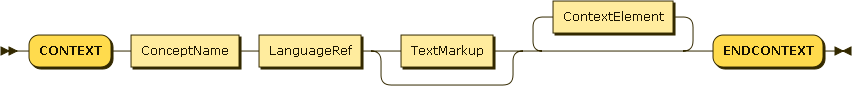
\includegraphics[resolution=120,max size={\textwidth}{\textheight}]{Figures/Ebnf/Context}
  \caption*{\texttt{Context \small::=  `CONTEXT' ConceptName LanguageRef TextMarkup? ContextElement* `ENDCONTEXT'}}
  \label{fig:ebnf-Context}
 \end{figure}

 \begin{figure}[H]
  \centering
  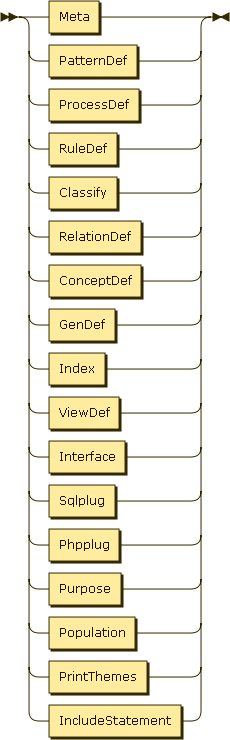
\includegraphics[resolution=120,max size={\textwidth}{\textheight}]{Figures/Ebnf/ContextElement}
  \caption*{\texttt{ContextElement \small::=  Meta | PatternDef | ProcessDef | RuleDef | Classify | RelationDef | ConceptDef | GenDef | Index | ViewDef | Interface | Sqlplug | Phpplug | Purpose | Population | PrintThemes | IncludeStatement}}
  \label{fig:ebnf-ContextElement}
 \end{figure}

 \begin{figure}[H]
  \centering
  
\includegraphics[resolution=120,max size={\textwidth}{\textheight}]{Figures/Ebnf/IncludeStatement}
  \caption*{\texttt{IncludeStatement \small::=  `INCLUDE' String}}
  \label{fig:ebnf-IncludeStatement}
 \end{figure}

 \begin{figure}[H]
  \centering
  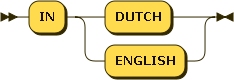
\includegraphics[resolution=120,max size={\textwidth}{\textheight}]{Figures/Ebnf/LanguageRef}
  \caption*{\texttt{LanguageRef \small::=  `IN' (`DUTCH' | `ENGLISH')}}
  \label{fig:ebnf-LanguageRef}
 \end{figure}

 \begin{figure}[H]
  \centering
  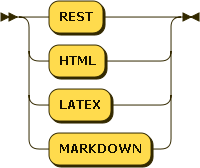
\includegraphics[resolution=120,max size={\textwidth}{\textheight}]{Figures/Ebnf/TextMarkup}
  \caption*{\texttt{TextMarkup \small::=  `REST' | `HTML' | `LATEX' | `MARKDOWN'}}
  \label{fig:ebnf-TextMarkup}
 \end{figure}

 \begin{figure}[H]
  \centering
  
\includegraphics[resolution=120,max size={\textwidth}{\textheight}]{Figures/Ebnf/Meta}
  \caption*{\texttt{Meta \small::=  `META' String String}}
  \label{fig:ebnf-Meta}
 \end{figure}

 \begin{figure}[H]
  \centering
  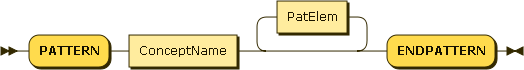
\includegraphics[resolution=120,max size={\textwidth}{\textheight}]{Figures/Ebnf/PatternDef}
  \caption*{\texttt{PatternDef \small::=  `PATTERN' ConceptName PatElem* `ENDPATTERN'}}
  \label{fig:ebnf-PatternDef}
 \end{figure}

 \begin{figure}[H]
  \centering
  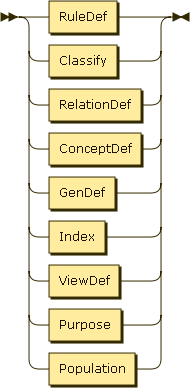
\includegraphics[resolution=120,max size={\textwidth}{\textheight}]{Figures/Ebnf/PatElem}
  \caption*{\texttt{PatElem \small::=  RuleDef | Classify | RelationDef | ConceptDef | GenDef | Index | ViewDef | Purpose | Population}}
  \label{fig:ebnf-PatElem}
 \end{figure}

 \begin{figure}[H]
  \centering
  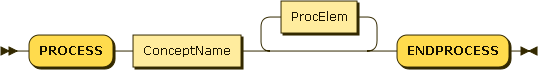
\includegraphics[resolution=120,max size={\textwidth}{\textheight}]{Figures/Ebnf/ProcessDef}
  \caption*{\texttt{ProcessDef \small::=  `PROCESS' ConceptName ProcElem* `ENDPROCESS'}}
  \label{fig:ebnf-ProcessDef}
 \end{figure}

 \begin{figure}[H]
  \centering
  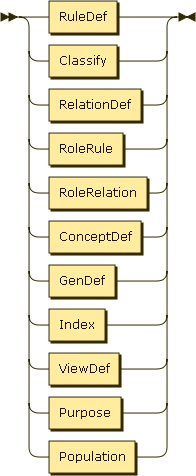
\includegraphics[resolution=120,max size={\textwidth}{\textheight}]{Figures/Ebnf/ProcElem}
  \caption*{\texttt{ProcElem \small::=  RuleDef | Classify | RelationDef | RoleRule | RoleRelation | ConceptDef | GenDef | Index | ViewDef | Purpose | Population}}
  \label{fig:ebnf-ProcElem}
 \end{figure}

 \begin{figure}[H]
  \centering
  
\includegraphics[resolution=120,max size={\textwidth}{\textheight}]{Figures/Ebnf/Classify}
  \caption*{\texttt{Classify \small::=  `CLASSIFY' ConceptRef `IS' Cterm}}
  \label{fig:ebnf-Classify}
 \end{figure}

 \begin{figure}[H]
  \centering
  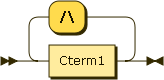
\includegraphics[resolution=120,max size={\textwidth}{\textheight}]{Figures/Ebnf/Cterm}
  \caption*{\texttt{Cterm \small::=  Cterm1 (`/\textbackslash{}' Cterm1)*}}
  \label{fig:ebnf-Cterm}
 \end{figure}

 \begin{figure}[H]
  \centering
  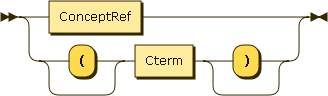
\includegraphics[resolution=120,max size={\textwidth}{\textheight}]{Figures/Ebnf/Cterm1}
  \caption*{\texttt{Cterm1 \small::=  ConceptRef | (`('? Cterm `)'?)}}
  \label{fig:ebnf-Cterm1}
 \end{figure}

 \begin{figure}[H]
  \centering
  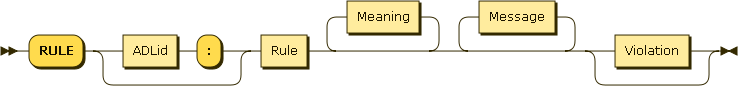
\includegraphics[resolution=120,max size={\textwidth}{\textheight}]{Figures/Ebnf/RuleDef}
  \caption*{\texttt{RuleDef \small::=  `RULE' (ADLid `:')? Rule Meaning* Message* Violation?}}
  \label{fig:ebnf-RuleDef}
 \end{figure}

 \begin{figure}[H]
  \centering
  
\includegraphics[resolution=120,max size={\textwidth}{\textheight}]{Figures/Ebnf/Violation}
  \caption*{\texttt{Violation \small::=  `VIOLATION' PairView}}
  \label{fig:ebnf-Violation}
 \end{figure}

 \begin{figure}[H]
  \centering
  
\includegraphics[resolution=120,max size={\textwidth}{\textheight}]{Figures/Ebnf/PairView}
  \caption*{\texttt{PairView \small::=  `(' PairViewSegmentList `)'}}
  \label{fig:ebnf-PairView}
 \end{figure}

 \begin{figure}[H]
  \centering
  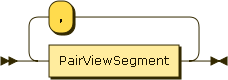
\includegraphics[resolution=120,max size={\textwidth}{\textheight}]{Figures/Ebnf/PairViewSegmentList}
  \caption*{\texttt{PairViewSegmentList \small::=  PairViewSegment (`,' PairViewSegment)*}}
  \label{fig:ebnf-PairViewSegmentList}
 \end{figure}

 \begin{figure}[H]
  \centering
  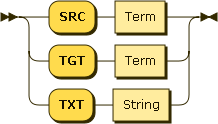
\includegraphics[resolution=120,max size={\textwidth}{\textheight}]{Figures/Ebnf/PairViewSegment}
  \caption*{\texttt{PairViewSegment \small::=  `SRC' Term | `TGT' Term | `TXT' String}}
  \label{fig:ebnf-PairViewSegment}
 \end{figure}

 \begin{figure}[H]
  \centering
  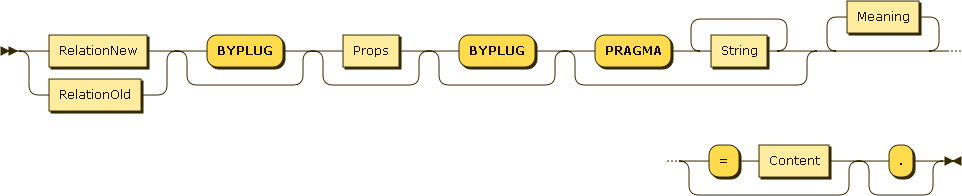
\includegraphics[resolution=120,max size={\textwidth}{\textheight}]{Figures/Ebnf/RelationDef}
  \caption*{\texttt{RelationDef \small::=  (RelationNew | RelationOld) `BYPLUG'? Props? `BYPLUG'? (`PRAGMA' String+)? Meaning* (`=' Content)? `.'?}}
  \label{fig:ebnf-RelationDef}
 \end{figure}

 \begin{figure}[H]
  \centering
  
\includegraphics[resolution=120,max size={\textwidth}{\textheight}]{Figures/Ebnf/RelationNew}
  \caption*{\texttt{RelationNew \small::=  `RELATION' Varid Sign}}
  \label{fig:ebnf-RelationNew}
 \end{figure}

 \begin{figure}[H]
  \centering
  
\includegraphics[resolution=120,max size={\textwidth}{\textheight}]{Figures/Ebnf/RelationOld}
  \caption*{\texttt{RelationOld \small::=  Varid `::' ConceptRef Fun ConceptRef}}
  \label{fig:ebnf-RelationOld}
 \end{figure}

 \begin{figure}[H]
  \centering
  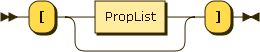
\includegraphics[resolution=120,max size={\textwidth}{\textheight}]{Figures/Ebnf/Props}
  \caption*{\texttt{Props \small::=  `[' PropList? `]'}}
  \label{fig:ebnf-Props}
 \end{figure}

 \begin{figure}[H]
  \centering
  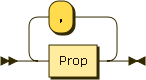
\includegraphics[resolution=120,max size={\textwidth}{\textheight}]{Figures/Ebnf/PropList}
  \caption*{\texttt{PropList \small::=  Prop (`,' Prop)*}}
  \label{fig:ebnf-PropList}
 \end{figure}

 \begin{figure}[H]
  \centering
  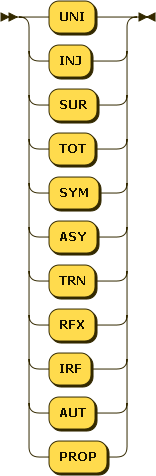
\includegraphics[resolution=120,max size={\textwidth}{\textheight}]{Figures/Ebnf/Prop}
  \caption*{\texttt{Prop \small::=  `UNI' | `INJ' | `SUR' | `TOT' | `SYM' | `ASY' | `TRN' | `RFX' | `IRF' | `AUT' | `PROP'}}
  \label{fig:ebnf-Prop}
 \end{figure}

 \begin{figure}[H]
  \centering
  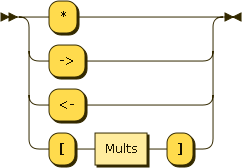
\includegraphics[resolution=120,max size={\textwidth}{\textheight}]{Figures/Ebnf/Fun}
  \caption*{\texttt{Fun \small::=  `*' | `->' | `<-' | `[' Mults `]'}}
  \label{fig:ebnf-Fun}
 \end{figure}

 \begin{figure}[H]
  \centering
  
\includegraphics[resolution=120,max size={\textwidth}{\textheight}]{Figures/Ebnf/Mults}
  \caption*{\texttt{Mults \small::=  Mult `-' Mult}}
  \label{fig:ebnf-Mults}
 \end{figure}

 \begin{figure}[H]
  \centering
  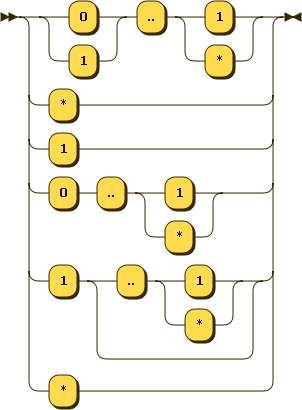
\includegraphics[resolution=120,max size={\textwidth}{\textheight}]{Figures/Ebnf/Mult}
  \caption*{\texttt{Mult \small::=  (`0' | `1') `..' (`1' | `*') | `*' | `1'}}
  \label{fig:ebnf-Mult}
 \end{figure}

 \begin{figure}[H]
  \centering
  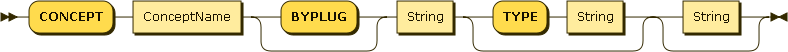
\includegraphics[resolution=120,max size={\textwidth}{\textheight}]{Figures/Ebnf/ConceptDef}
  \caption*{\texttt{ConceptDef \small::=  `CONCEPT' ConceptName `BYPLUG'? String (`TYPE' String)? String?}}
  \label{fig:ebnf-ConceptDef}
 \end{figure}

 \begin{figure}[H]
  \centering
  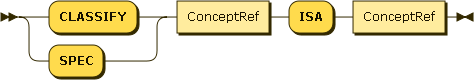
\includegraphics[resolution=120,max size={\textwidth}{\textheight}]{Figures/Ebnf/GenDef}
  \caption*{\texttt{GenDef \small::=  (`CLASSIFY' | `SPEC') ConceptRef `ISA' ConceptRef}}
  \label{fig:ebnf-GenDef}
 \end{figure}

 \begin{figure}[H]
  \centering
  
\includegraphics[resolution=120,max size={\textwidth}{\textheight}]{Figures/Ebnf/Index}
  \caption*{\texttt{Index \small::=  `IDENT' Label ConceptRefPos `(' IndSegmentList `)'}}
  \label{fig:ebnf-Index}
 \end{figure}

 \begin{figure}[H]
  \centering
  
\includegraphics[resolution=120,max size={\textwidth}{\textheight}]{Figures/Ebnf/IndSegmentList}
  \caption*{\texttt{IndSegmentList \small::=  IndSegment (`,' IndSegment)}}
  \label{fig:ebnf-IndSegmentList}
 \end{figure}

 \begin{figure}[H]
  \centering
  
\includegraphics[resolution=120,max size={\textwidth}{\textheight}]{Figures/Ebnf/IndSegment}
  \caption*{\texttt{IndSegment \small::=  IndAtt}}
  \label{fig:ebnf-IndSegment}
 \end{figure}

 \begin{figure}[H]
  \centering
  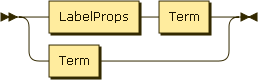
\includegraphics[resolution=120,max size={\textwidth}{\textheight}]{Figures/Ebnf/IndAtt}
  \caption*{\texttt{IndAtt \small::=  LabelProps Term | Term}}
  \label{fig:ebnf-IndAtt}
 \end{figure}

 \begin{figure}[H]
  \centering
  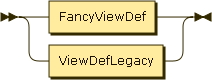
\includegraphics[resolution=120,max size={\textwidth}{\textheight}]{Figures/Ebnf/ViewDef}
  \caption*{\texttt{ViewDef \small::=  FancyViewDef | ViewDefLegacy}}
  \label{fig:ebnf-ViewDef}
 \end{figure}

 \begin{figure}[H]
  \centering
  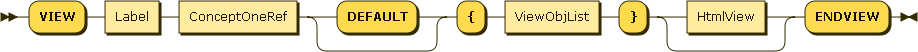
\includegraphics[resolution=120,max size={\textwidth}{\textheight}]{Figures/Ebnf/FancyViewDef}
  \caption*{\texttt{FancyViewDef \small::=  `VIEW' pLabel ConceptOneRefPos `DEFAULT'? `\{' ViewObjList `\}' HtmlView? `ENDVIEW'}}
  \label{fig:ebnf-FancyViewDef}
 \end{figure}

 \begin{figure}[H]
  \centering
  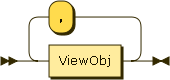
\includegraphics[resolution=120,max size={\textwidth}{\textheight}]{Figures/Ebnf/ViewObjList}
  \caption*{\texttt{ViewObjList \small::=  ViewObj (`,' ViewObj)*}}
  \label{fig:ebnf-ViewObjList}
 \end{figure}

 \begin{figure}[H]
  \centering
  
\includegraphics[resolution=120,max size={\textwidth}{\textheight}]{Figures/Ebnf/ViewObj}
  \caption*{\texttt{ViewObj \small::=  Label Term}}
  \label{fig:ebnf-ViewObj}
 \end{figure}

 \begin{figure}[H]
  \centering
  
\includegraphics[resolution=120,max size={\textwidth}{\textheight}]{Figures/Ebnf/HtmlView}
  \caption*{\texttt{HtmlView \small::=  `HTML' `TEMPLATE' String}}
  \label{fig:ebnf-HtmlView}
 \end{figure}

 \begin{figure}[H]
  \centering
  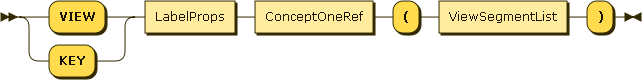
\includegraphics[resolution=120,max size={\textwidth}{\textheight}]{Figures/Ebnf/ViewDefLegacy}
  \caption*{\texttt{ViewDefLegacy \small::=  (`VIEW' | `KEY') LabelProps ConceptOneRefPos `(' ViewSegmentList `)'}}
  \label{fig:ebnf-ViewDefLegacy}
 \end{figure}

 \begin{figure}[H]
  \centering
  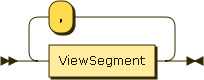
\includegraphics[resolution=120,max size={\textwidth}{\textheight}]{Figures/Ebnf/ViewSegmentList}
  \caption*{\texttt{ViewSegmentList \small::=  ViewSegment (`,' ViewSegment)*}}
  \label{fig:ebnf-ViewSegmentList}
 \end{figure}

 \begin{figure}[H]
  \centering
  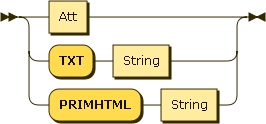
\includegraphics[resolution=120,max size={\textwidth}{\textheight}]{Figures/Ebnf/ViewSegment}
  \caption*{\texttt{ViewSegment \small::=  ViewAtt | `TXT' String | `PRIMHTML' String}}
  \label{fig:ebnf-ViewSegment}
 \end{figure}

 \begin{figure}[H]
  \centering
  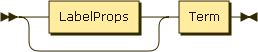
\includegraphics[resolution=120,max size={\textwidth}{\textheight}]{Figures/Ebnf/ViewAtt}
  \caption*{\texttt{ViewAtt \small::=  LabelProps? Term}}
  \label{fig:ebnf-ViewAtt}
 \end{figure}

 \begin{figure}[H]
  \centering
  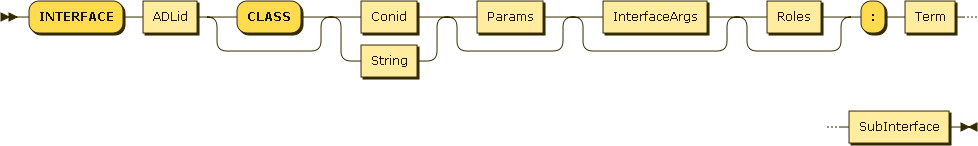
\includegraphics[resolution=120,max size={\textwidth}{\textheight}]{Figures/Ebnf/Interface}
  \caption*{\texttt{Interface \small::=  `INTERFACE' ADLid `CLASS'? (Conid | String) Params? InterfaceArgs? Roles? `:' Term SubInterface}}
  \label{fig:ebnf-Interface}
 \end{figure}

 \begin{figure}[H]
  \centering
  
\includegraphics[resolution=120,max size={\textwidth}{\textheight}]{Figures/Ebnf/Params}
  \caption*{\texttt{Params \small::=  `(' NamedRel `)'}}
  \label{fig:ebnf-Params}
 \end{figure}

 \begin{figure}[H]
  \centering
  
\includegraphics[resolution=120,max size={\textwidth}{\textheight}]{Figures/Ebnf/InterfaceArgs}
  \caption*{\texttt{InterfaceArgs \small::=  `\{' ADLidListList `\}'}}
  \label{fig:ebnf-InterfaceArgs}
 \end{figure}

 \begin{figure}[H]
  \centering
  
\includegraphics[resolution=120,max size={\textwidth}{\textheight}]{Figures/Ebnf/Roles}
  \caption*{\texttt{Roles \small::=  `FOR' RoleList}}
  \label{fig:ebnf-Roles}
 \end{figure}

 \begin{figure}[H]
  \centering
  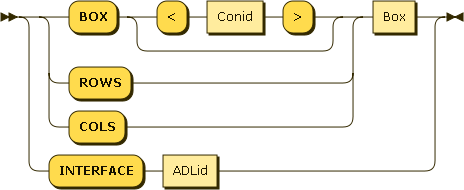
\includegraphics[resolution=120,max size={\textwidth}{\textheight}]{Figures/Ebnf/SubInterface}
  \caption*{\texttt{SubInterface \small::=  (`BOX' (`<' Conid `>')? | `ROWS' | `COLS') Box | `INTERFACE' ADLid}}
  \label{fig:ebnf-SubInterface}
 \end{figure}

 \begin{figure}[H]
  \centering
  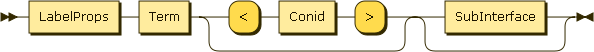
\includegraphics[resolution=120,max size={\textwidth}{\textheight}]{Figures/Ebnf/ObjDef}
  \caption*{\texttt{ObjDef \small::=  LabelProps Term (`<' Conid `>')? SubInterface?}}
  \label{fig:ebnf-ObjDef}
 \end{figure}

 \begin{figure}[H]
  \centering
  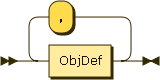
\includegraphics[resolution=120,max size={\textwidth}{\textheight}]{Figures/Ebnf/ObjDefList}
  \caption*{\texttt{ObjDefList \small::=  ObjDef (`,' ObjDef)*}}
  \label{fig:ebnf-ObjDefList}
 \end{figure}

 \begin{figure}[H]
  \centering
  \includegraphics[resolution=120,max size={\textwidth}{\textheight}]{Figures/Ebnf/Box}
  \caption*{\texttt{Box \small::=  `[' ObjDefList `]'}}
  \label{fig:ebnf-Box}
 \end{figure}

 \begin{figure}[H]
  \centering
  \includegraphics[resolution=120,max size={\textwidth}{\textheight}]{Figures/Ebnf/Sqlplug}
  \caption*{\texttt{Sqlplug \small::=  `SQLPLUG' ObjDef}}
  \label{fig:ebnf-Sqlplug}
 \end{figure}

 \begin{figure}[H]
  \centering
  \includegraphics[resolution=120,max size={\textwidth}{\textheight}]{Figures/Ebnf/Phpplug}
  \caption*{\texttt{Phpplug \small::=  `PHPPLUG' ObjDef}}
  \label{fig:ebnf-Phpplug}
 \end{figure}

 \begin{figure}[H]
  \centering
  \includegraphics[resolution=120,max size={\textwidth}{\textheight}]{Figures/Ebnf/Purpose}
  \caption*{\texttt{Purpose \small::=  `PURPOSE' Ref2Obj LanguageRef? TextMarkup? (`REF' StringListSemi)? Expl}}
  \label{fig:ebnf-Purpose}
 \end{figure}

 \begin{figure}[H]
  \centering
  \includegraphics[resolution=120,max size={\textwidth}{\textheight}]{Figures/Ebnf/Ref2Obj}
  \caption*{\texttt{Ref2Obj \small::=  `CONCEPT' ConceptName | `RELATION' RelSign | `RULE' ADLid | `IDENT' ADLid | `VIEW' ADLid | `PATTERN' ADLid | `PROCESS' ADLid | `INTERFACE' ADLid | `CONTEXT' ADLid}}
  \label{fig:ebnf-Ref2Obj}
 \end{figure}

 \begin{figure}[H]
  \centering
  \includegraphics[resolution=120,max size={\textwidth}{\textheight}]{Figures/Ebnf/Population}
  \caption*{\texttt{Population \small::=  `POPULATION' NamedRel `CONTAINS' Content | `POPULATION' ConceptName `CONTAINS' `[' ValueList `]'}}
  \label{fig:ebnf-Population}
 \end{figure}

 \begin{figure}[H]
  \centering
  \includegraphics[resolution=120,max size={\textwidth}{\textheight}]{Figures/Ebnf/RoleRelation}
  \caption*{\texttt{RoleRelation \small::=  `ROLE' RoleList `EDITS' NamedRelList}}
  \label{fig:ebnf-RoleRelation}
 \end{figure}

 \begin{figure}[H]
  \centering
  \includegraphics[resolution=120,max size={\textwidth}{\textheight}]{Figures/Ebnf/RoleRule}
  \caption*{\texttt{RoleRule \small::=  `ROLE' RoleList `MAINTAINS' ADLidList}}
  \label{fig:ebnf-RoleRule}
 \end{figure}

 \begin{figure}[H]
  \centering
  \includegraphics[resolution=120,max size={\textwidth}{\textheight}]{Figures/Ebnf/Role}
  \caption*{\texttt{Role \small::=  ADLid}}
  \label{fig:ebnf-Role}
 \end{figure}

 \begin{figure}[H]
  \centering
  \includegraphics[resolution=120,max size={\textwidth}{\textheight}]{Figures/Ebnf/RoleList}
  \caption*{\texttt{RoleList \small::=  Role (`,' Role)*}}
  \label{fig:ebnf-RoleList}
 \end{figure}

 \begin{figure}[H]
  \centering
  \includegraphics[resolution=120,max size={\textwidth}{\textheight}]{Figures/Ebnf/PrintThemes}
  \caption*{\texttt{PrintThemes \small::=  `THEMES' ConceptNameList}}
  \label{fig:ebnf-PrintThemes}
 \end{figure}

 \begin{figure}[H]
  \centering
  \includegraphics[resolution=120,max size={\textwidth}{\textheight}]{Figures/Ebnf/Meaning}
  \caption*{\texttt{Meaning \small::=  `MEANING' LanguageRef? TextMarkup? (String | Expl)}}
  \label{fig:ebnf-Meaning}
 \end{figure}

 \begin{figure}[H]
  \centering
  \includegraphics[resolution=120,max size={\textwidth}{\textheight}]{Figures/Ebnf/Message}
  \caption*{\texttt{Message \small::=  `MESSAGE' Markup}}
  \label{fig:ebnf-Message}
 \end{figure}

 \begin{figure}[H]
  \centering
  \includegraphics[resolution=120,max size={\textwidth}{\textheight}]{Figures/Ebnf/Rule}
  \caption*{\texttt{Rule \small::=  Term (`=' Term | `|-' Term)?}}
  \label{fig:ebnf-Rule}
 \end{figure}

 \begin{figure}[H]
  \centering
  \includegraphics[resolution=120,max size={\textwidth}{\textheight}]{Figures/Ebnf/Term}
  \caption*{\texttt{Term \small::=  Trm2 ((`/\textbackslash{}' Trm2)+ | (`\textbackslash{}/' Trm2)+)?}}
  \label{fig:ebnf-Term}
 \end{figure}

 \begin{figure}[H]
  \centering
  \includegraphics[resolution=120,max size={\textwidth}{\textheight}]{Figures/Ebnf/Trm2}
  \caption*{\texttt{Trm2 \small::=  Trm3 (`-' Trm3)?}}
  \label{fig:ebnf-Trm2}
 \end{figure}

 \begin{figure}[H]
  \centering
  \includegraphics[resolution=120,max size={\textwidth}{\textheight}]{Figures/Ebnf/Trm3}
  \caption*{\texttt{Trm3 \small::=  Trm4 (`/' Trm4 | `\textbackslash{}' Trm4 | `<>' Trm4)?}}
  \label{fig:ebnf-Trm3}
 \end{figure}

 \begin{figure}[H]
  \centering
  \includegraphics[resolution=120,max size={\textwidth}{\textheight}]{Figures/Ebnf/Trm4}
  \caption*{\texttt{Trm4 \small::=  Trm5 ((`;' Trm5)+ | (`!' Trm5)+ | (`\#' Trm5)+)?}}
  \label{fig:ebnf-Trm4}
 \end{figure}

 \begin{figure}[H]
  \centering
  \includegraphics[resolution=120,max size={\textwidth}{\textheight}]{Figures/Ebnf/Trm5}
  \caption*{\texttt{Trm5 \small::=  `-'* Trm6 (`~' | `*' | `+')*}}
  \label{fig:ebnf-Trm5}
 \end{figure}

 \begin{figure}[H]
  \centering
  \includegraphics[resolution=120,max size={\textwidth}{\textheight}]{Figures/Ebnf/Trm6}
  \caption*{\texttt{Trm6 \small::=  RelationRef | `(' Term `)'}}
  \label{fig:ebnf-Trm6}
 \end{figure}

 \begin{figure}[H]
  \centering
  \includegraphics[resolution=120,max size={\textwidth}{\textheight}]{Figures/Ebnf/RelationRef}
  \caption*{\texttt{RelationRef \small::=  RelSign | `I' (`[' ConceptOneRef `]')? | `V' Sign? | Atom (`[' ConceptOneRef `]')?}}
  \label{fig:ebnf-RelationRef}
 \end{figure}

 \begin{figure}[H]
  \centering
  \includegraphics[resolution=120,max size={\textwidth}{\textheight}]{Figures/Ebnf/NamedRelList}
  \caption*{\texttt{NamedRelList \small::=  NamedRel (`,' NamedRel)*}}
  \label{fig:ebnf-NamedRelList}
 \end{figure}

 \begin{figure}[H]
  \centering
  \includegraphics[resolution=120,max size={\textwidth}{\textheight}]{Figures/Ebnf/NamedRel}
  \caption*{\texttt{NamedRel \small::=  Varid Sign?}}
  \label{fig:ebnf-NamedRel}
 \end{figure}

 \begin{figure}[H]
  \centering
  \includegraphics[resolution=120,max size={\textwidth}{\textheight}]{Figures/Ebnf/Sign}
  \caption*{\texttt{Sign \small::=  `[' ConceptOneRef (`*' ConceptOneRef)? `]'}}
  \label{fig:ebnf-Sign}
 \end{figure}

 \begin{figure}[H]
  \centering
  \includegraphics[resolution=120,max size={\textwidth}{\textheight}]{Figures/Ebnf/ConceptName}
  \caption*{\texttt{ConceptName \small::=  Conid | String}}
  \label{fig:ebnf-ConceptName}
 \end{figure}

 \begin{figure}[H]
  \centering
  \includegraphics[resolution=120,max size={\textwidth}{\textheight}]{Figures/Ebnf/ConceptNameList}
  \caption*{\texttt{ConceptNameList \small::=  ConceptName (`,' ConceptName)}}
  \label{fig:ebnf-ConceptNameList}
 \end{figure}

 \begin{figure}[H]
  \centering
  \includegraphics[resolution=120,max size={\textwidth}{\textheight}]{Figures/Ebnf/ConceptRef}
  \caption*{\texttt{ConceptRef \small::=  ConceptName}}
  \label{fig:ebnf-ConceptRef}
 \end{figure}

 \begin{figure}[H]
  \centering
  \includegraphics[resolution=120,max size={\textwidth}{\textheight}]{Figures/Ebnf/ConceptOneRef}
  \caption*{\texttt{ConceptOneRef \small::=  `ONE' | ConceptRef}}
  \label{fig:ebnf-ConceptOneRef}
 \end{figure}

 \begin{figure}[H]
  \centering
  \includegraphics[resolution=120,max size={\textwidth}{\textheight}]{Figures/Ebnf/LabelProps}
  \caption*{\texttt{LabelProps \small::=  ADLid (`\{' ADLidListList `\}')? `:'}}
  \label{fig:ebnf-LabelProps}
 \end{figure}

 \begin{figure}[H]
  \centering
  \includegraphics[resolution=120,max size={\textwidth}{\textheight}]{Figures/Ebnf/Label}
  \caption*{\texttt{Label \small::=  ADLid `:'}}
  \label{fig:ebnf-Label}
 \end{figure}

 \begin{figure}[H]
  \centering
  \includegraphics[resolution=120,max size={\textwidth}{\textheight}]{Figures/Ebnf/Content}
  \caption*{\texttt{Content \small::=  `[' RecordList? `]' | `[' RecordObsList? `]'}}
  \label{fig:ebnf-Content}
 \end{figure}

 \begin{figure}[H]
  \centering
  \includegraphics[resolution=120,max size={\textwidth}{\textheight}]{Figures/Ebnf/RecordList}
  \caption*{\texttt{RecordList \small::=  Record (`,' Record)*}}
  \label{fig:ebnf-RecordList}
 \end{figure}

 \begin{figure}[H]
  \centering
  \includegraphics[resolution=120,max size={\textwidth}{\textheight}]{Figures/Ebnf/Record}
  \caption*{\texttt{Record \small::=  String `*' String}}
  \label{fig:ebnf-Record}
 \end{figure}

 \begin{figure}[H]
  \centering
  \includegraphics[resolution=120,max size={\textwidth}{\textheight}]{Figures/Ebnf/RecordObsList}
  \caption*{\texttt{RecordObsList \small::=  RecordObsList (`;' RecordObsList)}}
  \label{fig:ebnf-RecordObsList}
 \end{figure}

 \begin{figure}[H]
  \centering
  \includegraphics[resolution=120,max size={\textwidth}{\textheight}]{Figures/Ebnf/RecordObs}
  \caption*{\texttt{RecordObs \small::=  `(' String `,' String `)'}}
  \label{fig:ebnf-RecordObs}
 \end{figure}

 \begin{figure}[H]
  \centering
  \includegraphics[resolution=120,max size={\textwidth}{\textheight}]{Figures/Ebnf/ADLid}
  \caption*{\texttt{ADLid \small::=  Varid | Conid | String}}
  \label{fig:ebnf-ADLid}
 \end{figure}

 \begin{figure}[H]
  \centering
  \includegraphics[resolution=120,max size={\textwidth}{\textheight}]{Figures/Ebnf/ADLidList}
  \caption*{\texttt{ADLidList \small::=  ADLid (`,' ADLid)*}}
  \label{fig:ebnf-ADLidList}
 \end{figure}

 \begin{figure}[H]
  \centering
  \includegraphics[resolution=120,max size={\textwidth}{\textheight}]{Figures/Ebnf/ADLidListList}
  \caption*{\texttt{ADLidListList \small::=  ADLid+ (`,' ADLid+)*}}
  \label{fig:ebnf-ADLidListList}
 \end{figure}

 \begin{figure}[H]
  \centering
  \includegraphics[resolution=120,max size={\textwidth}{\textheight}]{Figures/Ebnf/Conid}
  \caption*{\texttt{Conid \small::=  UpperChar (Char | `\_')*}}
  \label{fig:ebnf-Conid}
 \end{figure}

 \begin{figure}[H]
  \centering
  \includegraphics[resolution=120,max size={\textwidth}{\textheight}]{Figures/Ebnf/String}
  \caption*{\texttt{String \small::=  `"' Any* `"'}}
  \label{fig:ebnf-String}
 \end{figure}

 \begin{figure}[H]
  \centering
  \includegraphics[resolution=120,max size={\textwidth}{\textheight}]{Figures/Ebnf/StringListSemi}
  \caption*{\texttt{StringListSemi \small::=  String (`;' String)*}}
  \label{fig:ebnf-StringListSemi}
 \end{figure}

 \begin{figure}[H]
  \centering
  \includegraphics[resolution=120,max size={\textwidth}{\textheight}]{Figures/Ebnf/Expl}
  \caption*{\texttt{Expl \small::=  `\{+' Any* `-\}'}}
  \label{fig:ebnf-Expl}
 \end{figure}

 \begin{figure}[H]
  \centering
  \includegraphics[resolution=120,max size={\textwidth}{\textheight}]{Figures/Ebnf/Varid}
  \caption*{\texttt{Varid \small::=  (LowerChar | `\_') (Char | `\_')*}}
  \label{fig:ebnf-Varid}
 \end{figure}


\newpage
\begin{landscape}

  \section*{Parse Tree}
  \label{app:parse-tree}
  \addcontentsline{toc}{section}{Parse Tree}
  \begin{figure}[htb!]
    \centering
    \includegraphics[width=25.4cm]{Figures/GenParseTree}
    \caption[Diagram of the Ampersand parse tree]{
      Diagram of the Ampersand parse tree. \small
      %Data definitions are depicted in green, constructors are depicted in blue and 
      Connections without an arrow represent the data contructors.
      Connections with an arrow also show the multiplicity in the relationship (i.e. 1 or *) or are stripped to represent an optional relationship.
      }
    \label{fig:parse-tree}
  \end{figure}

\end{landscape}
\newpage
\documentclass{book}
\usepackage{haddock}
\begin{document}
\begin{titlepage}
\begin{haddocktitle}

\end{haddocktitle}
\end{titlepage}
\tableofcontents
\haddockmoduleheading{Database.Design.Ampersand.ADL1.Pair}
\label{module:Database.Design.Ampersand.ADL1.Pair}
\haddockbeginheader
{\haddockverb\begin{verbatim}
module Database.Design.Ampersand.ADL1.Pair (
    Paire(Paire, srcPaire, trgPaire),  Pairs,  mkPair
  ) where\end{verbatim}}
\haddockendheader

\begin{haddockdesc}
\item[\begin{tabular}{@{}l}
data\ Paire
\end{tabular}]\haddockbegindoc
\haddockbeginconstrs
\haddockdecltt{=} & \haddockdecltt{Paire} & \\
                    \haddockdecltt{srcPaire :: String} &
                    \haddockdecltt{trgPaire :: String} &
\end{tabulary}\par
\end{haddockdesc}
\begin{haddockdesc}
\item[\begin{tabular}{@{}l}
instance\ Eq\ Paire\\instance\ Ord\ Paire\\instance\ Show\ Paire\\instance\ Unique\ Paire\\instance\ Typeable\ *\ Paire
\end{tabular}]
\end{haddockdesc}
\begin{haddockdesc}
\item[\begin{tabular}{@{}l}
type\ Pairs\ =\ {\char 91}Paire{\char 93}
\end{tabular}]
\end{haddockdesc}
\begin{haddockdesc}
\item[
mkPair\ ::\ String\ ->\ String\ ->\ Paire
]
\end{haddockdesc}
\haddockmoduleheading{Database.Design.Ampersand.Basics}
\label{module:Database.Design.Ampersand.Basics}
\haddockbeginheader
{\haddockverb\begin{verbatim}
module Database.Design.Ampersand.Basics (
    module Database.Design.Ampersand.Basics.Auxiliaries, 
    module Database.Design.Ampersand.Basics.Collection, 
    module Database.Design.Ampersand.Basics.String, 
    module Database.Design.Ampersand.Basics.Unique, 
    module Database.Design.Ampersand.Basics.UTF8, 
    module Database.Design.Ampersand.Basics.Version
  ) where\end{verbatim}}
\haddockendheader

\begin{haddockdesc}
\item[\begin{tabular}{@{}l}
module\ Database.Design.Ampersand.Basics.Auxiliaries\\module\ Database.Design.Ampersand.Basics.Collection\\module\ Database.Design.Ampersand.Basics.String\\module\ Database.Design.Ampersand.Basics.Unique\\module\ Database.Design.Ampersand.Basics.UTF8\\module\ Database.Design.Ampersand.Basics.Version
\end{tabular}]
\end{haddockdesc}
\haddockmoduleheading{Database.Design.Ampersand.Basics.Auxiliaries}
\label{module:Database.Design.Ampersand.Basics.Auxiliaries}
\haddockbeginheader
{\haddockverb\begin{verbatim}
module Database.Design.Ampersand.Basics.Auxiliaries (
    eqClass,  eqCl,  getCycles,  transClosureMap,  combinations,  converse, 
    commaEng,  commaNL,  fst3,  snd3,  thd3,  Flippable(flp),  showTrace, 
    showTraceTag,  blockParenthesize,  addToLastLine,  indent
  ) where\end{verbatim}}
\haddockendheader

\begin{haddockdesc}
\item[\begin{tabular}{@{}l}
eqClass\ ::\ (a\ ->\ a\ ->\ Bool)\ ->\ {\char 91}a{\char 93}\ ->\ {\char 91}{\char 91}a{\char 93}{\char 93}
\end{tabular}]\haddockbegindoc
The \haddockid{eqClass} function takes an equality test function and a list and returns a list of lists such

 that each sublist in the result contains only equal elements, and all equal elements are in

 the same sublist.  For example,
\par
Example> eqClass \haddocktt{Mississippi} = {\char 91}\haddocktt{M},"iiii","ssss","pp"{\char 93}
\par

\end{haddockdesc}
\begin{haddockdesc}
\item[\begin{tabular}{@{}l}
eqCl\ ::\ Eq\ b\ =>\ (a\ ->\ b)\ ->\ {\char 91}a{\char 93}\ ->\ {\char 91}{\char 91}a{\char 93}{\char 93}
\end{tabular}]\haddockbegindoc
eqCl is used for gathering things that are equal wrt some criterion f.

   For instance, if you want to have persons with the same name:

    'eqCl name persons' produces a list,in which each element is a list of persons with the same name.

 Example> eqCl (==\haddocktt{s}) \haddocktt{Mississippi} = "ssss"
\par

\end{haddockdesc}
\begin{haddockdesc}
\item[\begin{tabular}{@{}l}
getCycles\ ::\ Eq\ a\ =>\ {\char 91}(a,\ {\char 91}a{\char 93}){\char 93}\ ->\ {\char 91}{\char 91}a{\char 93}{\char 93}
\end{tabular}]\haddockbegindoc
getCycles returns a list of cycles in the edges list (each edge is a pair of a from-vertex

   and a list of to-vertices)
\par

\end{haddockdesc}
\begin{haddockdesc}
\item[\begin{tabular}{@{}l}
transClosureMap\ ::\ (Eq\ a,\ Ord\ a)\ =>\ Map\ a\ {\char 91}a{\char 93}\ ->\ Map\ a\ {\char 91}a{\char 93}
\end{tabular}]\haddockbegindoc
Warshall's transitive closure algorithm
\par

\end{haddockdesc}
\begin{haddockdesc}
\item[\begin{tabular}{@{}l}
combinations\ ::\ {\char 91}{\char 91}a{\char 93}{\char 93}\ ->\ {\char 91}{\char 91}a{\char 93}{\char 93}
\end{tabular}]\haddockbegindoc
The \haddockid{combinations} function returns all possible combinations of lists of list.

 For example,
\par
\begin{quote}
{\haddockverb\begin{verbatim}
combinations [[1,2,3],[10,20],[4]] == [[1,10,4],[1,20,4],[2,10,4],[2,20,4],[3,10,4],[3,20,4]]
\end{verbatim}}
\end{quote}

\end{haddockdesc}
\begin{haddockdesc}
\item[
converse\ ::\ forall\ a\ b.\ (Ord\ a,\ Ord\ b)\ =>\ {\char 91}(a,\ {\char 91}b{\char 93}){\char 93}\ ->\ {\char 91}(b,\ {\char 91}a{\char 93}){\char 93}
]
\item[
commaEng\ ::\ String\ ->\ {\char 91}String{\char 93}\ ->\ String
]
\item[
commaNL\ ::\ String\ ->\ {\char 91}String{\char 93}\ ->\ String
]
\item[
fst3\ ::\ (a,\ b,\ c)\ ->\ a
]
\item[
snd3\ ::\ (a,\ b,\ c)\ ->\ b
]
\item[
thd3\ ::\ (a,\ b,\ c)\ ->\ c
]
\end{haddockdesc}
\begin{haddockdesc}
\item[\begin{tabular}{@{}l}
class\ Flippable\ a\ where
\end{tabular}]\haddockbegindoc
\haddockpremethods{}\textbf{Methods}
\begin{haddockdesc}
\item[\begin{tabular}{@{}l}
flp\ ::\ a\ ->\ a
\end{tabular}]
\end{haddockdesc}
\end{haddockdesc}
\begin{haddockdesc}
\item[\begin{tabular}{@{}l}
instance\ Flippable\ Prop\\instance\ Flippable\ SrcOrTgt
\end{tabular}]
\end{haddockdesc}
\begin{haddockdesc}
\item[
showTrace\ ::\ Show\ a\ =>\ a\ ->\ a
]
\item[
showTraceTag\ ::\ Show\ a\ =>\ String\ ->\ a\ ->\ a
]
\item[
blockParenthesize\ ::\ String\\\ \ \ \ \ \ \ \ \ \ \ \ \ \ \ \ \ \ \ \ \ ->\ String\ ->\ String\ ->\ {\char 91}{\char 91}String{\char 93}{\char 93}\ ->\ {\char 91}String{\char 93}
]
\item[
addToLastLine\ ::\ String\ ->\ {\char 91}String{\char 93}\ ->\ {\char 91}String{\char 93}
]
\item[
indent\ ::\ Int\ ->\ {\char 91}String{\char 93}\ ->\ {\char 91}String{\char 93}
]
\end{haddockdesc}
\haddockmoduleheading{Database.Design.Ampersand.Basics.BuildInfo_Generated}
\label{module:Database.Design.Ampersand.Basics.BuildInfo_Generated}
\haddockbeginheader
{\haddockverb\begin{verbatim}
module Database.Design.Ampersand.Basics.BuildInfo_Generated (
    cabalVersionStr,  gitInfoStr,  buildTimeStr
  ) where\end{verbatim}}
\haddockendheader

\begin{haddockdesc}
\item[
cabalVersionStr\ ::\ String
]
\item[
gitInfoStr\ ::\ String
]
\item[
buildTimeStr\ ::\ String
]
\end{haddockdesc}
\haddockmoduleheading{Database.Design.Ampersand.Basics.Collection}
\label{module:Database.Design.Ampersand.Basics.Collection}
\haddockbeginheader
{\haddockverb\begin{verbatim}
module Database.Design.Ampersand.Basics.Collection (
    Collection(eleM, uni, isc, (>-), empty, elems)
  ) where\end{verbatim}}
\haddockendheader

\begin{haddockdesc}
\item[\begin{tabular}{@{}l}
class\ Collection\ a\ where
\end{tabular}]\haddockbegindoc
\haddockpremethods{}\textbf{Methods}
\begin{haddockdesc}
\item[\begin{tabular}{@{}l}
eleM\ ::\ Eq\ b\ =>\ b\ ->\ a\ b\ ->\ Bool
\end{tabular}]
\end{haddockdesc}
\begin{haddockdesc}
\item[\begin{tabular}{@{}l}
uni,\ isc\ ::\ Eq\ b\ =>\ a\ b\ ->\ a\ b\ ->\ a\ b
\end{tabular}]
\end{haddockdesc}
\begin{haddockdesc}
\item[\begin{tabular}{@{}l}
(>-)\ ::\ Eq\ b\ =>\ a\ b\ ->\ a\ b\ ->\ a\ b
\end{tabular}]
\end{haddockdesc}
\begin{haddockdesc}
\item[\begin{tabular}{@{}l}
empty\ ::\ Eq\ b\ =>\ a\ b
\end{tabular}]
\end{haddockdesc}
\begin{haddockdesc}
\item[\begin{tabular}{@{}l}
elems\ ::\ Eq\ b\ =>\ a\ b\ ->\ {\char 91}b{\char 93}
\end{tabular}]
\end{haddockdesc}
\end{haddockdesc}
\begin{haddockdesc}
\item[\begin{tabular}{@{}l}
instance\ Collection\ {\char 91}{\char 93}
\end{tabular}]
\end{haddockdesc}
\haddockmoduleheading{Database.Design.Ampersand.Basics.String}
\label{module:Database.Design.Ampersand.Basics.String}
\haddockbeginheader
{\haddockverb\begin{verbatim}
module Database.Design.Ampersand.Basics.String (
    unCap,  upCap,  escapeNonAlphaNum
  ) where\end{verbatim}}
\haddockendheader

This module contains some common String funcions
\par

\begin{haddockdesc}
\item[\begin{tabular}{@{}l}
unCap\ ::\ String\ ->\ String
\end{tabular}]\haddockbegindoc
Converts the first character of a string to lowercase, with the exception that there is a second character, which is uppercase.

 uncap \haddocktt{AbcDe} == "abcDe"

 uncap \haddocktt{ABcDE} == \haddocktt{ABcDE}
\par

\end{haddockdesc}
\begin{haddockdesc}
\item[\begin{tabular}{@{}l}
upCap\ ::\ String\ ->\ String
\end{tabular}]\haddockbegindoc
Converts the first character of a string to uppercase
\par

\end{haddockdesc}
\begin{haddockdesc}
\item[\begin{tabular}{@{}l}
escapeNonAlphaNum\ ::\ String\ ->\ String
\end{tabular}]\haddockbegindoc
escape anything except regular characters and digits to {\char '137}\href{character}{code}

 e.g. escapeNonAlphaNum "a{\char '137}�" = "a{\char '137}95{\char '137}233"
\par

\end{haddockdesc}
\haddockmoduleheading{Database.Design.Ampersand.Basics.UTF8}
\label{module:Database.Design.Ampersand.Basics.UTF8}
\haddockbeginheader
{\haddockverb\begin{verbatim}
module Database.Design.Ampersand.Basics.UTF8 (
    readUTF8File,  readFile,  writeFile,  getContents,  putStr,  putStrLn, 
    hGetContents,  hPutStr,  hPutStrLn
  ) where\end{verbatim}}
\haddockendheader

UTF-8 aware string IO functions that will work with GHC 6.10, 6.12, or 7.
\par

\begin{haddockdesc}
\item[
readUTF8File\ ::\ FilePath\ ->\ IO\ (Either\ String\ String)
]
\item[
readFile\ ::\ FilePath\ ->\ IO\ String
]
\item[
writeFile\ ::\ FilePath\ ->\ String\ ->\ IO\ ()
]
\item[
getContents\ ::\ IO\ String
]
\item[
putStr\ ::\ String\ ->\ IO\ ()
]
\item[
putStrLn\ ::\ String\ ->\ IO\ ()
]
\item[
hGetContents\ ::\ Handle\ ->\ IO\ String
]
\item[
hPutStr\ ::\ Handle\ ->\ String\ ->\ IO\ ()
]
\item[
hPutStrLn\ ::\ Handle\ ->\ String\ ->\ IO\ ()
]
\end{haddockdesc}
\haddockmoduleheading{Database.Design.Ampersand.Basics.Unique}
\label{module:Database.Design.Ampersand.Basics.Unique}
\haddockbeginheader
{\haddockverb\begin{verbatim}
module Database.Design.Ampersand.Basics.Unique (
    Unique(self, uniqueShow, showUnique),  Named(name)
  ) where\end{verbatim}}
\haddockendheader

\begin{haddockdesc}
\item[\begin{tabular}{@{}l}
class\ (Typeable\ e,\ Eq\ e)\ =>\ Unique\ e\ where
\end{tabular}]\haddockbegindoc
In the context of the haskell code, things can be Unique. 
\par

\haddockpremethods{}\textbf{Methods}
\begin{haddockdesc}
\item[\begin{tabular}{@{}l}
self\ ::\ e\ ->\ UniqueObj\ e
\end{tabular}]\haddockbegindoc
a representation of a unique thing
\par

\end{haddockdesc}
\begin{haddockdesc}
\item[\begin{tabular}{@{}l}
uniqueShow\ ::\ Bool\ ->\ e\ ->\ String
\end{tabular}]\haddockbegindoc
representation of a Unique thing into a string.  
\par

\end{haddockdesc}
\begin{haddockdesc}
\item[\begin{tabular}{@{}l}
showUnique\ ::\ e\ ->\ String
\end{tabular}]\haddockbegindoc
A function to show a unique instance. It is the responsability

   of the instance definition to make sure that for every a, b of 

   an individual type:

        a == b  \url{==} showUnique a == showUnique b
\par

\end{haddockdesc}
\end{haddockdesc}
\begin{haddockdesc}
\item[\begin{tabular}{@{}l}
instance\ Unique\ Bool\\instance\ Unique\ Origin\\instance\ Unique\ Paire\\instance\ Unique\ ConceptDef\\instance\ Unique\ Role\\instance\ Unique\ a\ =>\ Unique\ {\char 91}a{\char 93}
\end{tabular}]
\end{haddockdesc}
\begin{haddockdesc}
\item[\begin{tabular}{@{}l}
class\ Named\ a\ where
\end{tabular}]\haddockbegindoc
anything could have some label, can't it?
\par

\haddockpremethods{}\textbf{Methods}
\begin{haddockdesc}
\item[\begin{tabular}{@{}l}
name\ ::\ a\ ->\ String
\end{tabular}]
\end{haddockdesc}
\end{haddockdesc}
\begin{haddockdesc}
\item[\begin{tabular}{@{}l}
instance\ Named\ P{\char '137}Concept\\instance\ Named\ PPurpose\\instance\ Named\ PRef2Obj\\instance\ Named\ P{\char '137}Interface\\instance\ Named\ P{\char '137}Population\\instance\ Named\ P{\char '137}NamedRel\\instance\ Named\ TermPrim\\instance\ Named\ P{\char '137}Declaration\\instance\ Named\ ConceptDef\\instance\ Named\ P{\char '137}Pattern\\instance\ Named\ Role\\instance\ Named\ P{\char '137}Context\\instance\ Named\ (P{\char '137}ViewD\ a)\\instance\ Named\ (P{\char '137}IdentDf\ a)\\instance\ Named\ (P{\char '137}ObjDef\ a)\\instance\ Named\ (P{\char '137}Rule\ a)
\end{tabular}]
\end{haddockdesc}
\haddockmoduleheading{Database.Design.Ampersand.Basics.Version}
\label{module:Database.Design.Ampersand.Basics.Version}
\haddockbeginheader
{\haddockverb\begin{verbatim}
module Database.Design.Ampersand.Basics.Version (
    ampersandVersionStr,  ampersandVersionWithoutBuildTimeStr,  fatalMsg
  ) where\end{verbatim}}
\haddockendheader

This module contains Version of Ampersand
\par

\begin{haddockdesc}
\item[\begin{tabular}{@{}l}
ampersandVersionStr\ ::\ String
\end{tabular}]\haddockbegindoc
String, containing the Ampersand version, including the build timestamp.
\par

\end{haddockdesc}
\begin{haddockdesc}
\item[\begin{tabular}{@{}l}
ampersandVersionWithoutBuildTimeStr\ ::\ String
\end{tabular}]\haddockbegindoc
String, containing the Ampersand version
\par

\end{haddockdesc}
\begin{haddockdesc}
\item[\begin{tabular}{@{}l}
fatalMsg\ ::\ String\ ->\ Int\ ->\ String\ ->\ a
\end{tabular}]\haddockbegindoc
a function to create error message in a structured way, containing the version of Ampersand.

   It throws an error, showing a (module)name and a number. This makes debugging pretty easy.
\par

\end{haddockdesc}
\haddockmoduleheading{Database.Design.Ampersand.Core.ParseTree}
\label{module:Database.Design.Ampersand.Core.ParseTree}
\haddockbeginheader
{\haddockverb\begin{verbatim}
module Database.Design.Ampersand.Core.ParseTree (
    P_Context(PCtx,
              ctx_nm,
              ctx_pos,
              ctx_lang,
              ctx_markup,
              ctx_thms,
              ctx_pats,
              ctx_rs,
              ctx_ds,
              ctx_cs,
              ctx_ks,
              ctx_rrules,
              ctx_rrels,
              ctx_vs,
              ctx_gs,
              ctx_ifcs,
              ctx_ps,
              ctx_pops,
              ctx_sql,
              ctx_php,
              ctx_metas), 
    mergeContexts,  Meta(Meta, mtPos, mtObj, mtName, mtVal), 
    MetaObj(ContextMeta),  P_RoleRelation(P_RR, rr_Pos, rr_Roles, rr_Rels), 
    P_RoleRule(Maintain, mPos, mRoles, mRules),  Role(Role), 
    P_Pattern(P_Pat,
              pt_pos,
              pt_nm,
              pt_rls,
              pt_gns,
              pt_dcs,
              pt_RRuls,
              pt_RRels,
              pt_cds,
              pt_ids,
              pt_vds,
              pt_xps,
              pt_pop,
              pt_end), 
    P_Declaration(P_Sgn,
                  dec_nm,
                  dec_sign,
                  dec_prps,
                  dec_pragma,
                  dec_Mean,
                  dec_popu,
                  dec_fpos,
                  dec_plug), 
    Term(Prim,
         PEqu,
         PImp,
         PIsc,
         PUni,
         PDif,
         PLrs,
         PRrs,
         PDia,
         PCps,
         PRad,
         PPrd,
         PKl0,
         PKl1,
         PFlp,
         PCpl,
         PBrk), 
    TermPrim(PI, Pid, Patm, PVee, Pfull, PNamedR),  P_NamedRel(PNamedRel), 
    PairView(PairView, ppv_segs), 
    PairViewSegment(PairViewText,
                    PairViewExp,
                    pvsOrg,
                    pvsStr,
                    pvsOrg,
                    pvsSoT,
                    pvsExp), 
    PairViewTerm(PairViewTerm),  PairViewSegmentTerm(PairViewSegmentTerm), 
    SrcOrTgt(Src, Tgt),  isSrc, 
    P_Rule(P_Ru, rr_fps, rr_nm, rr_exp, rr_mean, rr_msg, rr_viol), 
    ConceptDef(Cd, cdpos, cdcpt, cdplug, cddef, cdtyp, cdref, cdfrom), 
    P_Population(P_RelPopu,
                 P_TRelPop,
                 P_CptPopu,
                 p_orig,
                 p_rnme,
                 p_popps,
                 p_orig,
                 p_rnme,
                 p_type,
                 p_popps,
                 p_orig,
                 p_cnme,
                 p_popas), 
    P_ObjectDef,  P_SubInterface, 
    P_Interface(P_Ifc,
                ifc_Name,
                ifc_Class,
                ifc_Params,
                ifc_Args,
                ifc_Roles,
                ifc_Obj,
                ifc_Pos,
                ifc_Prp), 
    P_IClass(P_IClass, iclass_name), 
    P_ObjDef(P_Obj, obj_nm, obj_pos, obj_ctx, obj_mView, obj_msub, obj_strs), 
    P_SubIfc(P_Box, P_InterfaceRef, si_ori, si_class, si_box, si_ori, si_str), 
    P_IdentDef,  P_IdentDf(P_Id, ix_pos, ix_lbl, ix_cpt, ix_ats), 
    P_IdentSegment,  P_IdentSegmnt(P_IdentExp, ks_obj),  P_ViewDef, 
    P_ViewSegment,  ViewHtmlTemplate(ViewHtmlTemplateFile), 
    P_ViewD(P_Vd, vd_pos, vd_lbl, vd_cpt, vd_isDefault, vd_html, vd_ats), 
    P_ViewSegmt(P_ViewExp, P_ViewText, P_ViewHtml, vs_obj, vs_txt, vs_htm), 
    PPurpose(PRef2, pexPos, pexObj, pexMarkup, pexRefIDs), 
    PRef2Obj(PRef2ConceptDef,
             PRef2Declaration,
             PRef2Rule,
             PRef2IdentityDef,
             PRef2ViewDef,
             PRef2Pattern,
             PRef2Interface,
             PRef2Context,
             PRef2Fspc), 
    PMeaning(PMeaning),  PMessage(PMessage), 
    P_Concept(PCpt, P_Singleton, p_cptnm),  P_Sign(P_Sign, pSrc, pTgt), 
    P_Gen(P_Cy, PGen, gen_fp, gen_spc, gen_rhs, gen_fp, gen_spc, gen_gen), 
    Lang(Dutch, English),  P_Markup(P_Markup, mLang, mFormat, mString), 
    PandocFormat(HTML, ReST, LaTeX, Markdown), 
    Prop(Uni, Inj, Sur, Tot, Sym, Asy, Trn, Rfx, Irf, Aut, Prop),  Props, 
    normalizeProps,  module Database.Design.Ampersand.Input.ADL1.FilePos, 
    module Database.Design.Ampersand.ADL1.Pair,  gen_concs
  ) where\end{verbatim}}
\haddockendheader

\begin{haddockdesc}
\item[\begin{tabular}{@{}l}
data\ P{\char '137}Context
\end{tabular}]\haddockbegindoc
\haddockbeginconstrs
\haddockdecltt{=} & \haddockdecltt{PCtx} & \\
                    \haddockdecltt{ctx_nm :: String} & The name of this context

                    \haddockdecltt{ctx_pos :: [Origin]} & The origin of the context. A context can be a merge of a file including other files c.q. a list of Origin.

                    \haddockdecltt{ctx_lang :: Lang} & The default language specified on the top-level context

                    \haddockdecltt{ctx_markup :: Maybe PandocFormat} & The default markup format for free text in this context

                    \haddockdecltt{ctx_thms :: [String]} & Names of patterns/processes to be printed in the functional specification. (For partial documents.)

                    \haddockdecltt{ctx_pats :: [P_Pattern]} & The patterns defined in this context

                    \haddockdecltt{ctx_rs :: [P_Rule TermPrim]} & All user defined rules in this context, but outside patterns and outside processes

                    \haddockdecltt{ctx_ds :: [P_Declaration]} & The relations defined in this context, outside the scope of patterns

                    \haddockdecltt{ctx_cs :: [ConceptDef]} & The concept definitions defined in this context, outside the scope of patterns

                    \haddockdecltt{ctx_ks :: [P_IdentDef]} & The identity definitions defined in this context, outside the scope of patterns

                    \haddockdecltt{ctx_rrules :: [P_RoleRule]} & The MAINTAIN definitions defined in this context, outside the scope of patterns

                    \haddockdecltt{ctx_rrels :: [P_RoleRelation]} & The assignment of roles to Relations. (EDITS statements)

                    \haddockdecltt{ctx_vs :: [P_ViewDef]} & The view definitions defined in this context, outside the scope of patterns

                    \haddockdecltt{ctx_gs :: [P_Gen]} & The gen definitions defined in this context, outside the scope of patterns

                    \haddockdecltt{ctx_ifcs :: [P_Interface]} & The interfaces defined in this context

                    \haddockdecltt{ctx_ps :: [PPurpose]} & The purposes defined in this context, outside the scope of patterns and processes

                    \haddockdecltt{ctx_pops :: [P_Population]} & The populations defined in this context

                    \haddockdecltt{ctx_sql :: [P_ObjectDef]} & user defined sqlplugs, taken from the Ampersand script

                    \haddockdecltt{ctx_php :: [P_ObjectDef]} & user defined phpplugs, taken from the Ampersand script

                    \haddockdecltt{ctx_metas :: [Meta]} & generic meta information (name/value pairs) that can be used for experimenting without having to modify the adl syntax

\end{tabulary}\par
\end{haddockdesc}
\begin{haddockdesc}
\item[\begin{tabular}{@{}l}
instance\ Eq\ P{\char '137}Context\\instance\ Show\ P{\char '137}Context\\instance\ Named\ P{\char '137}Context
\end{tabular}]
\end{haddockdesc}
\begin{haddockdesc}
\item[
mergeContexts\ ::\ P{\char '137}Context\ ->\ P{\char '137}Context\ ->\ P{\char '137}Context
]
\end{haddockdesc}
\begin{haddockdesc}
\item[\begin{tabular}{@{}l}
data\ Meta
\end{tabular}]\haddockbegindoc
\haddockbeginconstrs
\haddockdecltt{=} & \haddockdecltt{Meta} & \\
                    \haddockdecltt{mtPos :: Origin} &
                    \haddockdecltt{mtObj :: MetaObj} &
                    \haddockdecltt{mtName :: String} &
                    \haddockdecltt{mtVal :: String} &
\end{tabulary}\par
\end{haddockdesc}
\begin{haddockdesc}
\item[\begin{tabular}{@{}l}
instance\ Show\ Meta
\end{tabular}]
\end{haddockdesc}
\begin{haddockdesc}
\item[\begin{tabular}{@{}l}
data\ MetaObj
\end{tabular}]\haddockbegindoc
\haddockbeginconstrs
\haddockdecltt{=} & \haddockdecltt{ContextMeta} & \\
\end{tabulary}\par
\end{haddockdesc}
\begin{haddockdesc}
\item[\begin{tabular}{@{}l}
instance\ Show\ MetaObj
\end{tabular}]
\end{haddockdesc}
\begin{haddockdesc}
\item[\begin{tabular}{@{}l}
data\ P{\char '137}RoleRelation
\end{tabular}]\haddockbegindoc
\haddockbeginconstrs
\haddockdecltt{=} & \haddockdecltt{P_RR} & \\
                    \haddockdecltt{rr_Pos :: Origin} & position in the Ampersand script

                    \haddockdecltt{rr_Roles :: [Role]} & list of roles

                    \haddockdecltt{rr_Rels :: [P_NamedRel]} & list of named relations

\end{tabulary}\par
A RoleRelation rs means that any role in 'rrRoles rs' may edit any Relation  in  'rrInterfaces rs'
\par

\end{haddockdesc}
\begin{haddockdesc}
\item[\begin{tabular}{@{}l}
instance\ Eq\ P{\char '137}RoleRelation\\instance\ Show\ P{\char '137}RoleRelation\\instance\ Traced\ P{\char '137}RoleRelation
\end{tabular}]
\end{haddockdesc}
\begin{haddockdesc}
\item[\begin{tabular}{@{}l}
data\ P{\char '137}RoleRule
\end{tabular}]\haddockbegindoc
\haddockbeginconstrs
\haddockdecltt{=} & \haddockdecltt{Maintain} & \\
                    \haddockdecltt{mPos :: Origin} & position in the Ampersand script

                    \haddockdecltt{mRoles :: [Role]} & name of a role

                    \haddockdecltt{mRules :: [String]} & name of a Rule

\end{tabulary}\par
\end{haddockdesc}
\begin{haddockdesc}
\item[\begin{tabular}{@{}l}
instance\ Eq\ P{\char '137}RoleRule\\instance\ Show\ P{\char '137}RoleRule\\instance\ Traced\ P{\char '137}RoleRule
\end{tabular}]
\end{haddockdesc}
\begin{haddockdesc}
\item[\begin{tabular}{@{}l}
data\ Role
\end{tabular}]\haddockbegindoc
\haddockbeginconstrs
\haddockdecltt{=} & \haddockdecltt{Role String} & \\
\end{tabulary}\par
\end{haddockdesc}
\begin{haddockdesc}
\item[\begin{tabular}{@{}l}
instance\ Eq\ Role\\instance\ Show\ Role\\instance\ Unique\ Role\\instance\ Named\ Role\\instance\ Typeable\ *\ Role
\end{tabular}]
\end{haddockdesc}
\begin{haddockdesc}
\item[\begin{tabular}{@{}l}
data\ P{\char '137}Pattern
\end{tabular}]\haddockbegindoc
\haddockbeginconstrs
\haddockdecltt{=} & \haddockdecltt{P_Pat} & \\
                    \haddockdecltt{pt_pos :: Origin} & the starting position in the file in which this pattern was declared.

                    \haddockdecltt{pt_nm :: String} & Name of this pattern

                    \haddockdecltt{pt_rls :: [P_Rule TermPrim]} & The user defined rules in this pattern

                    \haddockdecltt{pt_gns :: [P_Gen]} & The generalizations defined in this pattern

                    \haddockdecltt{pt_dcs :: [P_Declaration]} & The relations that are declared in this pattern

                    \haddockdecltt{pt_RRuls :: [P_RoleRule]} & The assignment of roles to rules.

                    \haddockdecltt{pt_RRels :: [P_RoleRelation]} & The assignment of roles to Relations.

                    \haddockdecltt{pt_cds :: [ConceptDef]} & The concept definitions defined in this pattern

                    \haddockdecltt{pt_ids :: [P_IdentDef]} & The identity definitions defined in this pattern

                    \haddockdecltt{pt_vds :: [P_ViewDef]} & The view definitions defined in this pattern

                    \haddockdecltt{pt_xps :: [PPurpose]} & The purposes of elements defined in this pattern

                    \haddockdecltt{pt_pop :: [P_Population]} & The populations that are local to this pattern

                    \haddockdecltt{pt_end :: Origin} & the end position in the file in which this pattern was declared.

\end{tabulary}\par
\end{haddockdesc}
\begin{haddockdesc}
\item[\begin{tabular}{@{}l}
instance\ Show\ P{\char '137}Pattern\\instance\ Named\ P{\char '137}Pattern\\instance\ Traced\ P{\char '137}Pattern
\end{tabular}]
\end{haddockdesc}
\begin{haddockdesc}
\item[\begin{tabular}{@{}l}
data\ P{\char '137}Declaration
\end{tabular}]\haddockbegindoc
\haddockbeginconstrs
\haddockdecltt{=} & \haddockdecltt{P_Sgn} & \\
                    \haddockdecltt{dec_nm :: String} & the name of the declaration

                    \haddockdecltt{dec_sign :: P_Sign} & the type. Parser must guarantee it is not empty.

                    \haddockdecltt{dec_prps :: Props} & the user defined multiplicity properties (Uni, Tot, Sur, Inj) and algebraic properties (Sym, Asy, Trn, Rfx)

                    \haddockdecltt{dec_pragma :: [String]} & Three strings, which form the pragma. E.g. if pragma consists of the three strings: "Person ", " is married to person ", and " in Vegas."

 {\char '136}    then a tuple (\haddocktt{Peter},\haddocktt{Jane}) in the list of links means that Person Peter is married to person Jane in Vegas.

                    \haddockdecltt{dec_Mean :: [PMeaning]} & the optional meaning of a declaration, possibly more than one for different languages.

                    \haddockdecltt{dec_popu :: Pairs} & the list of tuples, of which the relation consists.

                    \haddockdecltt{dec_fpos :: Origin} & the position in the Ampersand source file where this declaration is declared. Not all decalartions come from the ampersand souce file.

                    \haddockdecltt{dec_plug :: Bool} & if true, this relation may not be stored in or retrieved from the standard database (it should be gotten from a Plug of some sort instead)

\end{tabulary}\par
\end{haddockdesc}
\begin{haddockdesc}
\item[\begin{tabular}{@{}l}
instance\ Eq\ P{\char '137}Declaration\\instance\ Ord\ P{\char '137}Declaration\\instance\ Show\ P{\char '137}Declaration\\instance\ Named\ P{\char '137}Declaration\\instance\ Traced\ P{\char '137}Declaration
\end{tabular}]
\end{haddockdesc}
\begin{haddockdesc}
\item[\begin{tabular}{@{}l}
data\ Term\ a
\end{tabular}]\haddockbegindoc
\haddockbeginconstrs
\haddockdecltt{=} & \haddockdecltt{Prim a} & \\
\haddockdecltt{|} & \haddockdecltt{PEqu Origin (Term a) (Term a)} & equivalence             =
 \\
\haddockdecltt{|} & \haddockdecltt{PImp Origin (Term a) (Term a)} & implication             |-
 \\
\haddockdecltt{|} & \haddockdecltt{PIsc Origin (Term a) (Term a)} & intersection            /
 \\
\haddockdecltt{|} & \haddockdecltt{PUni Origin (Term a) (Term a)} & union                   /
 \\
\haddockdecltt{|} & \haddockdecltt{PDif Origin (Term a) (Term a)} & difference              -
 \\
\haddockdecltt{|} & \haddockdecltt{PLrs Origin (Term a) (Term a)} & left residual           /
 \\
\haddockdecltt{|} & \haddockdecltt{PRrs Origin (Term a) (Term a)} & right residual          
 \\
\haddockdecltt{|} & \haddockdecltt{PDia Origin (Term a) (Term a)} & diamond                 <>
 \\
\haddockdecltt{|} & \haddockdecltt{PCps Origin (Term a) (Term a)} & composition             ;
 \\
\haddockdecltt{|} & \haddockdecltt{PRad Origin (Term a) (Term a)} & relative addition       !
 \\
\haddockdecltt{|} & \haddockdecltt{PPrd Origin (Term a) (Term a)} & cartesian product       *
 \\
\haddockdecltt{|} & \haddockdecltt{PKl0 Origin (Term a)} & Rfx.Trn closure         *  (Kleene star)
 \\
\haddockdecltt{|} & \haddockdecltt{PKl1 Origin (Term a)} & Transitive closure      +  (Kleene plus)
 \\
\haddockdecltt{|} & \haddockdecltt{PFlp Origin (Term a)} & conversion (flip, wok)  {\char '176}
 \\
\haddockdecltt{|} & \haddockdecltt{PCpl Origin (Term a)} & Complement
 \\
\haddockdecltt{|} & \haddockdecltt{PBrk Origin (Term a)} & bracketed expression ( ... )
 \\
\end{tabulary}\par
\end{haddockdesc}
\begin{haddockdesc}
\item[\begin{tabular}{@{}l}
instance\ Functor\ Term\\instance\ Foldable\ Term\\instance\ Traversable\ Term\\instance\ Show\ a\ =>\ Show\ (Term\ a)\\instance\ Traced\ a\ =>\ Traced\ (Term\ a)
\end{tabular}]
\end{haddockdesc}
\begin{haddockdesc}
\item[\begin{tabular}{@{}l}
data\ TermPrim
\end{tabular}]\haddockbegindoc
\haddockbeginconstrs
\haddockdecltt{=} & \haddockdecltt{PI Origin} & identity element without a type

   At parse time, there may be zero or one element in the list of concepts.

   Reason: when making eqClasses, the least element of that class is used as a witness of that class

   to know whether an eqClass represents a concept, we only look at its witness

   By making Pid the first in the data decleration, it becomes the least element for "deriving Ord".
 \\
\haddockdecltt{|} & \haddockdecltt{Pid Origin P_Concept} & identity element restricted to a type
 \\
\haddockdecltt{|} & \haddockdecltt{Patm Origin String (Maybe P_Concept)} & an atom, possibly with a type
 \\
\haddockdecltt{|} & \haddockdecltt{PVee Origin} & the complete relation, of which the type is yet to be derived by the type checker.
 \\
\haddockdecltt{|} & \haddockdecltt{Pfull Origin P_Concept P_Concept} & the complete relation, restricted to a type.

   At parse time, there may be zero, one or two elements in the list of concepts.
 \\
\haddockdecltt{|} & \haddockdecltt{PNamedR P_NamedRel} & \\
\end{tabulary}\par
\end{haddockdesc}
\begin{haddockdesc}
\item[\begin{tabular}{@{}l}
instance\ Show\ TermPrim\\instance\ Named\ TermPrim\\instance\ Traced\ TermPrim
\end{tabular}]
\end{haddockdesc}
\begin{haddockdesc}
\item[\begin{tabular}{@{}l}
data\ P{\char '137}NamedRel
\end{tabular}]\haddockbegindoc
\haddockbeginconstrs
\haddockdecltt{=} & \haddockdecltt{PNamedRel Origin String (Maybe P_Sign)} & \\
\end{tabulary}\par
\end{haddockdesc}
\begin{haddockdesc}
\item[\begin{tabular}{@{}l}
instance\ Show\ P{\char '137}NamedRel\\instance\ Named\ P{\char '137}NamedRel\\instance\ Traced\ P{\char '137}NamedRel
\end{tabular}]
\end{haddockdesc}
\begin{haddockdesc}
\item[\begin{tabular}{@{}l}
data\ PairView\ a
\end{tabular}]\haddockbegindoc
\haddockbeginconstrs
\haddockdecltt{=} & \haddockdecltt{PairView} & \\
                    \haddockdecltt{ppv_segs :: [PairViewSegment a]} &
\end{tabulary}\par
\end{haddockdesc}
\begin{haddockdesc}
\item[\begin{tabular}{@{}l}
instance\ Functor\ PairView\\instance\ Foldable\ PairView\\instance\ Traversable\ PairView\\instance\ Eq\ a\ =>\ Eq\ (PairView\ a)\\instance\ Show\ a\ =>\ Show\ (PairView\ a)\\instance\ Generic\ (PairView\ a)\\instance\ Hashable\ a\ =>\ Hashable\ (PairView\ a)\\instance\ Traced\ a\ =>\ Traced\ (PairView\ a)\\instance\ Typeable\ (*\ ->\ *)\ PairView\\instance\ type\ Rep\ (PairView\ a)
\end{tabular}]
\end{haddockdesc}
\begin{haddockdesc}
\item[\begin{tabular}{@{}l}
data\ PairViewSegment\ a
\end{tabular}]\haddockbegindoc
\haddockbeginconstrs
\haddockdecltt{=} & \haddockdecltt{PairViewText} & \\
                    \haddockdecltt{pvsOrg :: Origin} &
                    \haddockdecltt{pvsStr :: String} &
\haddockdecltt{|} & \haddockdecltt{PairViewExp} & \\
                    \haddockdecltt{pvsOrg :: Origin} &
                    \haddockdecltt{pvsSoT :: SrcOrTgt} &
                    \haddockdecltt{pvsExp :: a} &
\end{tabulary}\par
\end{haddockdesc}
\begin{haddockdesc}
\item[\begin{tabular}{@{}l}
instance\ Functor\ PairViewSegment\\instance\ Foldable\ PairViewSegment\\instance\ Traversable\ PairViewSegment\\instance\ Eq\ a\ =>\ Eq\ (PairViewSegment\ a)\\instance\ Show\ a\ =>\ Show\ (PairViewSegment\ a)\\instance\ Generic\ (PairViewSegment\ a)\\instance\ Hashable\ a\ =>\ Hashable\ (PairViewSegment\ a)\\instance\ Traced\ (PairViewSegment\ a)\\instance\ Typeable\ (*\ ->\ *)\ PairViewSegment\\instance\ type\ Rep\ (PairViewSegment\ a)
\end{tabular}]
\end{haddockdesc}
\begin{haddockdesc}
\item[\begin{tabular}{@{}l}
newtype\ PairViewTerm\ a
\end{tabular}]\haddockbegindoc
\haddockbeginconstrs
\haddockdecltt{=} & \haddockdecltt{PairViewTerm (PairView (Term a))} & \\
\end{tabulary}\par
the newtype to make it possible for a PairView to be disambiguatable: it must be of the form "d a" instead of "d (Term a)"
\par

\end{haddockdesc}
\begin{haddockdesc}
\item[\begin{tabular}{@{}l}
instance\ Functor\ PairViewTerm\\instance\ Foldable\ PairViewTerm\\instance\ Traversable\ PairViewTerm
\end{tabular}]
\end{haddockdesc}
\begin{haddockdesc}
\item[\begin{tabular}{@{}l}
newtype\ PairViewSegmentTerm\ a
\end{tabular}]\haddockbegindoc
\haddockbeginconstrs
\haddockdecltt{=} & \haddockdecltt{PairViewSegmentTerm (PairViewSegment (Term a))} & \\
\end{tabulary}\par
\end{haddockdesc}
\begin{haddockdesc}
\item[\begin{tabular}{@{}l}
instance\ Functor\ PairViewSegmentTerm\\instance\ Foldable\ PairViewSegmentTerm\\instance\ Traversable\ PairViewSegmentTerm
\end{tabular}]
\end{haddockdesc}
\begin{haddockdesc}
\item[\begin{tabular}{@{}l}
data\ SrcOrTgt
\end{tabular}]\haddockbegindoc
\haddockbeginconstrs
\haddockdecltt{=} & \haddockdecltt{Src} & \\
\haddockdecltt{|} & \haddockdecltt{Tgt} & \\
\end{tabulary}\par
\end{haddockdesc}
\begin{haddockdesc}
\item[\begin{tabular}{@{}l}
instance\ Eq\ SrcOrTgt\\instance\ Ord\ SrcOrTgt\\instance\ Show\ SrcOrTgt\\instance\ Generic\ SrcOrTgt\\instance\ Flippable\ SrcOrTgt\\instance\ Hashable\ SrcOrTgt\\instance\ type\ Rep\ SrcOrTgt
\end{tabular}]
\end{haddockdesc}
\begin{haddockdesc}
\item[
isSrc\ ::\ SrcOrTgt\ ->\ Bool
]
\end{haddockdesc}
\begin{haddockdesc}
\item[\begin{tabular}{@{}l}
data\ P{\char '137}Rule\ a
\end{tabular}]\haddockbegindoc
\haddockbeginconstrs
\haddockdecltt{=} & \haddockdecltt{P_Ru} & \\
                    \haddockdecltt{rr_fps :: Origin} & Position in the Ampersand file

                    \haddockdecltt{rr_nm :: String} & Name of this rule

                    \haddockdecltt{rr_exp :: Term a} & The rule expression

                    \haddockdecltt{rr_mean :: [PMeaning]} & User-specified meanings, possibly more than one, for multiple languages.

                    \haddockdecltt{rr_msg :: [PMessage]} & User-specified violation messages, possibly more than one, for multiple languages.

                    \haddockdecltt{rr_viol :: Maybe (PairView (Term a))} & Custom presentation for violations, currently only in a single language

\end{tabulary}\par
\end{haddockdesc}
\begin{haddockdesc}
\item[\begin{tabular}{@{}l}
instance\ Functor\ P{\char '137}Rule\\instance\ Foldable\ P{\char '137}Rule\\instance\ Traversable\ P{\char '137}Rule\\instance\ Show\ a\ =>\ Show\ (P{\char '137}Rule\ a)\\instance\ Named\ (P{\char '137}Rule\ a)\\instance\ Traced\ (P{\char '137}Rule\ a)
\end{tabular}]
\end{haddockdesc}
\begin{haddockdesc}
\item[\begin{tabular}{@{}l}
data\ ConceptDef
\end{tabular}]\haddockbegindoc
\haddockbeginconstrs
\haddockdecltt{=} & \haddockdecltt{Cd} & \\
                    \haddockdecltt{cdpos :: Origin} & The position of this definition in the text of the Ampersand source (filename, line number and column number).

                    \haddockdecltt{cdcpt :: String} & The name of the concept for which this is the definition. If there is no such concept, the conceptdefinition is ignored.

                    \haddockdecltt{cdplug :: Bool} & Whether the user specifically told Ampersand not to store this concept in the database

                    \haddockdecltt{cddef :: String} & The textual definition of this concept.

                    \haddockdecltt{cdtyp :: String} & The (SQL) type of this concept.

                    \haddockdecltt{cdref :: String} & A label meant to identify the source of the definition. (useful as LaTeX' symbolic reference)

                    \haddockdecltt{cdfrom :: String} & The name of the pattern or context in which this concept definition was made

\end{tabulary}\par
\end{haddockdesc}
\begin{haddockdesc}
\item[\begin{tabular}{@{}l}
instance\ Eq\ ConceptDef\\instance\ Show\ ConceptDef\\instance\ Unique\ ConceptDef\\instance\ Named\ ConceptDef\\instance\ Traced\ ConceptDef\\instance\ Typeable\ *\ ConceptDef
\end{tabular}]
\end{haddockdesc}
\begin{haddockdesc}
\item[\begin{tabular}{@{}l}
data\ P{\char '137}Population
\end{tabular}]\haddockbegindoc
\haddockbeginconstrs
\haddockdecltt{=} & \haddockdecltt{P_RelPopu} & \\
                    \haddockdecltt{p_orig :: Origin} &
                    \haddockdecltt{p_rnme :: String} &
                    \haddockdecltt{p_popps :: Pairs} &
\haddockdecltt{|} & \haddockdecltt{P_TRelPop} & \\
                    \haddockdecltt{p_orig :: Origin} &
                    \haddockdecltt{p_rnme :: String} &
                    \haddockdecltt{p_type :: P_Sign} &
                    \haddockdecltt{p_popps :: Pairs} &
\haddockdecltt{|} & \haddockdecltt{P_CptPopu} & \\
                    \haddockdecltt{p_orig :: Origin} &
                    \haddockdecltt{p_cnme :: String} &
                    \haddockdecltt{p_popas :: [String]} &
\end{tabulary}\par
\end{haddockdesc}
\begin{haddockdesc}
\item[\begin{tabular}{@{}l}
instance\ Show\ P{\char '137}Population\\instance\ Named\ P{\char '137}Population\\instance\ Traced\ P{\char '137}Population
\end{tabular}]
\end{haddockdesc}
\begin{haddockdesc}
\item[\begin{tabular}{@{}l}
type\ P{\char '137}ObjectDef\ =\ P{\char '137}ObjDef\ TermPrim
\end{tabular}]
\end{haddockdesc}
\begin{haddockdesc}
\item[\begin{tabular}{@{}l}
type\ P{\char '137}SubInterface\ =\ P{\char '137}SubIfc\ TermPrim
\end{tabular}]
\end{haddockdesc}
\begin{haddockdesc}
\item[\begin{tabular}{@{}l}
data\ P{\char '137}Interface
\end{tabular}]\haddockbegindoc
\haddockbeginconstrs
\haddockdecltt{=} & \haddockdecltt{P_Ifc} & \\
                    \haddockdecltt{ifc_Name :: String} & the name of the interface

                    \haddockdecltt{ifc_Class :: Maybe String} & the class of the interface

                    \haddockdecltt{ifc_Params :: [P_NamedRel]} & a list of named relations that are editable within this interface.

                    \haddockdecltt{ifc_Args :: [[String]]} & a list of arguments for code generation.

                    \haddockdecltt{ifc_Roles :: [Role]} & a list of roles that may use this interface

                    \haddockdecltt{ifc_Obj :: P_ObjectDef} & the context expression (mostly: I{\char 91}c{\char 93})

                    \haddockdecltt{ifc_Pos :: Origin} &
                    \haddockdecltt{ifc_Prp :: String} &
\end{tabulary}\par
\end{haddockdesc}
\begin{haddockdesc}
\item[\begin{tabular}{@{}l}
instance\ Show\ P{\char '137}Interface\\instance\ Named\ P{\char '137}Interface\\instance\ Traced\ P{\char '137}Interface
\end{tabular}]
\end{haddockdesc}
\begin{haddockdesc}
\item[\begin{tabular}{@{}l}
data\ P{\char '137}IClass
\end{tabular}]\haddockbegindoc
\haddockbeginconstrs
\haddockdecltt{=} & \haddockdecltt{P_IClass} & \\
                    \haddockdecltt{iclass_name :: String} &
\end{tabulary}\par
\end{haddockdesc}
\begin{haddockdesc}
\item[\begin{tabular}{@{}l}
instance\ Eq\ P{\char '137}IClass\\instance\ Show\ P{\char '137}IClass
\end{tabular}]
\end{haddockdesc}
\begin{haddockdesc}
\item[\begin{tabular}{@{}l}
data\ P{\char '137}ObjDef\ a
\end{tabular}]\haddockbegindoc
\haddockbeginconstrs
\haddockdecltt{=} & \haddockdecltt{P_Obj} & \\
                    \haddockdecltt{obj_nm :: String} & view name of the object definition. The label has no meaning in the Compliant Service Layer, but is used in the generated user interface if it is not an empty string.

                    \haddockdecltt{obj_pos :: Origin} & position of this definition in the text of the Ampersand source file (filename, line number and column number)

                    \haddockdecltt{obj_ctx :: Term a} & this expression describes the instances of this object, related to their context.

                    \haddockdecltt{obj_mView :: Maybe String} & The view that should be used for this object

                    \haddockdecltt{obj_msub :: Maybe (P_SubIfc a)} & the attributes, which are object definitions themselves.

                    \haddockdecltt{obj_strs :: [[String]]} & directives that specify the interface.

\end{tabulary}\par
\end{haddockdesc}
\begin{haddockdesc}
\item[\begin{tabular}{@{}l}
instance\ Functor\ P{\char '137}ObjDef\\instance\ Foldable\ P{\char '137}ObjDef\\instance\ Traversable\ P{\char '137}ObjDef\\instance\ Eq\ (P{\char '137}ObjDef\ a)\\instance\ Show\ a\ =>\ Show\ (P{\char '137}ObjDef\ a)\\instance\ Named\ (P{\char '137}ObjDef\ a)\\instance\ Traced\ (P{\char '137}ObjDef\ a)
\end{tabular}]
\end{haddockdesc}
\begin{haddockdesc}
\item[\begin{tabular}{@{}l}
data\ P{\char '137}SubIfc\ a
\end{tabular}]\haddockbegindoc
\haddockbeginconstrs
\haddockdecltt{=} & \haddockdecltt{P_Box} & \\
                    \haddockdecltt{si_ori :: Origin} &
                    \haddockdecltt{si_class :: Maybe String} &
                    \haddockdecltt{si_box :: [P_ObjDef a]} &
\haddockdecltt{|} & \haddockdecltt{P_InterfaceRef} & \\
                    \haddockdecltt{si_ori :: Origin} &
                    \haddockdecltt{si_str :: String} &
\end{tabulary}\par
\end{haddockdesc}
\begin{haddockdesc}
\item[\begin{tabular}{@{}l}
instance\ Functor\ P{\char '137}SubIfc\\instance\ Foldable\ P{\char '137}SubIfc\\instance\ Traversable\ P{\char '137}SubIfc\\instance\ Eq\ (P{\char '137}SubIfc\ a)\\instance\ Show\ a\ =>\ Show\ (P{\char '137}SubIfc\ a)\\instance\ Traced\ (P{\char '137}SubIfc\ a)
\end{tabular}]
\end{haddockdesc}
\begin{haddockdesc}
\item[\begin{tabular}{@{}l}
type\ P{\char '137}IdentDef\ =\ P{\char '137}IdentDf\ TermPrim
\end{tabular}]
\end{haddockdesc}
\begin{haddockdesc}
\item[\begin{tabular}{@{}l}
data\ P{\char '137}IdentDf\ a
\end{tabular}]\haddockbegindoc
\haddockbeginconstrs
\haddockdecltt{=} & \haddockdecltt{P_Id} & \\
                    \haddockdecltt{ix_pos :: Origin} & position of this definition in the text of the Ampersand source file (filename, line number and column number).

                    \haddockdecltt{ix_lbl :: String} & the name (or label) of this Identity. The label has no meaning in the Compliant Service Layer, but is used in the generated user interface. It is not an empty string.

                    \haddockdecltt{ix_cpt :: P_Concept} & this expression describes the instances of this object, related to their context

                    \haddockdecltt{ix_ats :: [P_IdentSegmnt a]} & the constituent segments of this identity. TODO: refactor to a list of terms

\end{tabulary}\par
\end{haddockdesc}
\begin{haddockdesc}
\item[\begin{tabular}{@{}l}
instance\ Functor\ P{\char '137}IdentDf\\instance\ Foldable\ P{\char '137}IdentDf\\instance\ Traversable\ P{\char '137}IdentDf\\instance\ Eq\ (P{\char '137}IdentDf\ a)\\instance\ Show\ a\ =>\ Show\ (P{\char '137}IdentDf\ a)\\instance\ Named\ (P{\char '137}IdentDf\ a)\\instance\ Traced\ (P{\char '137}IdentDf\ a)
\end{tabular}]
\end{haddockdesc}
\begin{haddockdesc}
\item[\begin{tabular}{@{}l}
type\ P{\char '137}IdentSegment\ =\ P{\char '137}IdentSegmnt\ TermPrim
\end{tabular}]
\end{haddockdesc}
\begin{haddockdesc}
\item[\begin{tabular}{@{}l}
data\ P{\char '137}IdentSegmnt\ a
\end{tabular}]\haddockbegindoc
\haddockbeginconstrs
\haddockdecltt{=} & \haddockdecltt{P_IdentExp} & \\
                    \haddockdecltt{ks_obj :: P_ObjDef a} &
\end{tabulary}\par
\end{haddockdesc}
\begin{haddockdesc}
\item[\begin{tabular}{@{}l}
instance\ Functor\ P{\char '137}IdentSegmnt\\instance\ Foldable\ P{\char '137}IdentSegmnt\\instance\ Traversable\ P{\char '137}IdentSegmnt\\instance\ Eq\ (P{\char '137}IdentSegmnt\ a)\\instance\ Show\ a\ =>\ Show\ (P{\char '137}IdentSegmnt\ a)
\end{tabular}]
\end{haddockdesc}
\begin{haddockdesc}
\item[\begin{tabular}{@{}l}
type\ P{\char '137}ViewDef\ =\ P{\char '137}ViewD\ TermPrim
\end{tabular}]
\end{haddockdesc}
\begin{haddockdesc}
\item[\begin{tabular}{@{}l}
type\ P{\char '137}ViewSegment\ =\ P{\char '137}ViewSegmt\ TermPrim
\end{tabular}]
\end{haddockdesc}
\begin{haddockdesc}
\item[\begin{tabular}{@{}l}
data\ ViewHtmlTemplate
\end{tabular}]\haddockbegindoc
\haddockbeginconstrs
\haddockdecltt{=} & \haddockdecltt{ViewHtmlTemplateFile String} & \\
\end{tabulary}\par
\end{haddockdesc}
\begin{haddockdesc}
\item[\begin{tabular}{@{}l}
instance\ Eq\ ViewHtmlTemplate\\instance\ Show\ ViewHtmlTemplate
\end{tabular}]
\end{haddockdesc}
\begin{haddockdesc}
\item[\begin{tabular}{@{}l}
data\ P{\char '137}ViewD\ a
\end{tabular}]\haddockbegindoc
\haddockbeginconstrs
\haddockdecltt{=} & \haddockdecltt{P_Vd} & \\
                    \haddockdecltt{vd_pos :: Origin} & position of this definition in the text of the Ampersand source file (filename, line number and column number).

                    \haddockdecltt{vd_lbl :: String} & the name (or label) of this View. The label has no meaning in the Compliant Service Layer, but is used in the generated user interface. It is not an empty string.

                    \haddockdecltt{vd_cpt :: P_Concept} & the concept for which this view is applicable

                    \haddockdecltt{vd_isDefault :: Bool} & whether or not this is the default view for the concept 

                    \haddockdecltt{vd_html :: Maybe ViewHtmlTemplate} & the html template for this view (not required since we may have other kinds of views as well in the future)

              , vd{\char '137}text :: Maybe P{\char '137}ViewText -- Future extension

                    \haddockdecltt{vd_ats :: [P_ViewSegmt a]} & the constituent segments of this view.

\end{tabulary}\par
\end{haddockdesc}
\begin{haddockdesc}
\item[\begin{tabular}{@{}l}
instance\ Functor\ P{\char '137}ViewD\\instance\ Foldable\ P{\char '137}ViewD\\instance\ Traversable\ P{\char '137}ViewD\\instance\ Show\ a\ =>\ Show\ (P{\char '137}ViewD\ a)\\instance\ Named\ (P{\char '137}ViewD\ a)\\instance\ Traced\ (P{\char '137}ViewD\ a)
\end{tabular}]
\end{haddockdesc}
\begin{haddockdesc}
\item[\begin{tabular}{@{}l}
data\ P{\char '137}ViewSegmt\ a
\end{tabular}]\haddockbegindoc
\haddockbeginconstrs
\haddockdecltt{=} & \haddockdecltt{P_ViewExp} & \\
                    \haddockdecltt{vs_obj :: P_ObjDef a} &
\haddockdecltt{|} & \haddockdecltt{P_ViewText} & \\
                    \haddockdecltt{vs_txt :: String} &
\haddockdecltt{|} & \haddockdecltt{P_ViewHtml} & \\
                    \haddockdecltt{vs_htm :: String} &
\end{tabulary}\par
\end{haddockdesc}
\begin{haddockdesc}
\item[\begin{tabular}{@{}l}
instance\ Functor\ P{\char '137}ViewSegmt\\instance\ Foldable\ P{\char '137}ViewSegmt\\instance\ Traversable\ P{\char '137}ViewSegmt\\instance\ Eq\ (P{\char '137}ViewSegmt\ a)\\instance\ Show\ a\ =>\ Show\ (P{\char '137}ViewSegmt\ a)
\end{tabular}]
\end{haddockdesc}
\begin{haddockdesc}
\item[\begin{tabular}{@{}l}
data\ PPurpose
\end{tabular}]\haddockbegindoc
\haddockbeginconstrs
\haddockdecltt{=} & \haddockdecltt{PRef2} & \\
                    \haddockdecltt{pexPos :: Origin} &
                    \haddockdecltt{pexObj :: PRef2Obj} &
                    \haddockdecltt{pexMarkup :: P_Markup} &
                    \haddockdecltt{pexRefIDs :: [String]} &
\end{tabulary}\par
\end{haddockdesc}
\begin{haddockdesc}
\item[\begin{tabular}{@{}l}
instance\ Show\ PPurpose\\instance\ Named\ PPurpose\\instance\ Traced\ PPurpose
\end{tabular}]
\end{haddockdesc}
\begin{haddockdesc}
\item[\begin{tabular}{@{}l}
data\ PRef2Obj
\end{tabular}]\haddockbegindoc
\haddockbeginconstrs
\haddockdecltt{=} & \haddockdecltt{PRef2ConceptDef String} & \\
\haddockdecltt{|} & \haddockdecltt{PRef2Declaration P_NamedRel} & \\
\haddockdecltt{|} & \haddockdecltt{PRef2Rule String} & \\
\haddockdecltt{|} & \haddockdecltt{PRef2IdentityDef String} & \\
\haddockdecltt{|} & \haddockdecltt{PRef2ViewDef String} & \\
\haddockdecltt{|} & \haddockdecltt{PRef2Pattern String} & \\
\haddockdecltt{|} & \haddockdecltt{PRef2Interface String} & \\
\haddockdecltt{|} & \haddockdecltt{PRef2Context String} & \\
\haddockdecltt{|} & \haddockdecltt{PRef2Fspc String} & \\
\end{tabulary}\par
\end{haddockdesc}
\begin{haddockdesc}
\item[\begin{tabular}{@{}l}
instance\ Show\ PRef2Obj\\instance\ Named\ PRef2Obj
\end{tabular}]
\end{haddockdesc}
\begin{haddockdesc}
\item[\begin{tabular}{@{}l}
newtype\ PMeaning
\end{tabular}]\haddockbegindoc
\haddockbeginconstrs
\haddockdecltt{=} & \haddockdecltt{PMeaning P_Markup} & \\
\end{tabulary}\par
\end{haddockdesc}
\begin{haddockdesc}
\item[\begin{tabular}{@{}l}
instance\ Show\ PMeaning
\end{tabular}]
\end{haddockdesc}
\begin{haddockdesc}
\item[\begin{tabular}{@{}l}
newtype\ PMessage
\end{tabular}]\haddockbegindoc
\haddockbeginconstrs
\haddockdecltt{=} & \haddockdecltt{PMessage P_Markup} & \\
\end{tabulary}\par
\end{haddockdesc}
\begin{haddockdesc}
\item[\begin{tabular}{@{}l}
instance\ Show\ PMessage
\end{tabular}]
\end{haddockdesc}
\begin{haddockdesc}
\item[\begin{tabular}{@{}l}
data\ P{\char '137}Concept
\end{tabular}]\haddockbegindoc
\haddockbeginconstrs
\haddockdecltt{=} & \haddockdecltt{PCpt} & The name of this Concept
 \\
                    \haddockdecltt{p_cptnm :: String} &
\haddockdecltt{|} & \haddockdecltt{P_Singleton} & \\
\end{tabulary}\par
\end{haddockdesc}
\begin{haddockdesc}
\item[\begin{tabular}{@{}l}
instance\ Show\ P{\char '137}Concept\\instance\ Named\ P{\char '137}Concept
\end{tabular}]
\end{haddockdesc}
\begin{haddockdesc}
\item[\begin{tabular}{@{}l}
data\ P{\char '137}Sign
\end{tabular}]\haddockbegindoc
\haddockbeginconstrs
\haddockdecltt{=} & \haddockdecltt{P_Sign} & \\
                    \haddockdecltt{pSrc :: P_Concept} &
                    \haddockdecltt{pTgt :: P_Concept} &
\end{tabulary}\par
\end{haddockdesc}
\begin{haddockdesc}
\item[\begin{tabular}{@{}l}
instance\ Show\ P{\char '137}Sign
\end{tabular}]
\end{haddockdesc}
\begin{haddockdesc}
\item[\begin{tabular}{@{}l}
data\ P{\char '137}Gen
\end{tabular}]\haddockbegindoc
\haddockbeginconstrs
\haddockdecltt{=} & \haddockdecltt{P_Cy} & \\
                    \haddockdecltt{gen_fp :: Origin} & Position in the Ampersand file

                    \haddockdecltt{gen_spc :: P_Concept} & Left hand side concept expression

                    \haddockdecltt{gen_rhs :: [P_Concept]} & Right hand side concept expression

\haddockdecltt{|} & \haddockdecltt{PGen} & \\
                    \haddockdecltt{gen_fp :: Origin} & Position in the Ampersand file

                    \haddockdecltt{gen_spc :: P_Concept} & Left hand side concept expression

                    \haddockdecltt{gen_gen :: P_Concept} & generic concept

\end{tabulary}\par
\end{haddockdesc}
\begin{haddockdesc}
\item[\begin{tabular}{@{}l}
instance\ Show\ P{\char '137}Gen\\instance\ Traced\ P{\char '137}Gen
\end{tabular}]
\end{haddockdesc}
\begin{haddockdesc}
\item[\begin{tabular}{@{}l}
data\ Lang
\end{tabular}]\haddockbegindoc
\haddockbeginconstrs
\haddockdecltt{=} & \haddockdecltt{Dutch} & \\
\haddockdecltt{|} & \haddockdecltt{English} & \\
\end{tabulary}\par
\end{haddockdesc}
\begin{haddockdesc}
\item[\begin{tabular}{@{}l}
instance\ Eq\ Lang\\instance\ Ord\ Lang\\instance\ Show\ Lang
\end{tabular}]
\end{haddockdesc}
\begin{haddockdesc}
\item[\begin{tabular}{@{}l}
data\ P{\char '137}Markup
\end{tabular}]\haddockbegindoc
\haddockbeginconstrs
\haddockdecltt{=} & \haddockdecltt{P_Markup} & \\
                    \haddockdecltt{mLang :: Maybe Lang} &
                    \haddockdecltt{mFormat :: Maybe PandocFormat} &
                    \haddockdecltt{mString :: String} &
\end{tabulary}\par
\end{haddockdesc}
\begin{haddockdesc}
\item[\begin{tabular}{@{}l}
instance\ Show\ P{\char '137}Markup
\end{tabular}]
\end{haddockdesc}
\begin{haddockdesc}
\item[\begin{tabular}{@{}l}
data\ PandocFormat
\end{tabular}]\haddockbegindoc
\haddockbeginconstrs
\haddockdecltt{=} & \haddockdecltt{HTML} & \\
\haddockdecltt{|} & \haddockdecltt{ReST} & \\
\haddockdecltt{|} & \haddockdecltt{LaTeX} & \\
\haddockdecltt{|} & \haddockdecltt{Markdown} & \\
\end{tabulary}\par
\end{haddockdesc}
\begin{haddockdesc}
\item[\begin{tabular}{@{}l}
instance\ Eq\ PandocFormat\\instance\ Ord\ PandocFormat\\instance\ Show\ PandocFormat
\end{tabular}]
\end{haddockdesc}
\begin{haddockdesc}
\item[\begin{tabular}{@{}l}
data\ Prop
\end{tabular}]\haddockbegindoc
\haddockbeginconstrs
\haddockdecltt{=} & \haddockdecltt{Uni} & univalent
 \\
\haddockdecltt{|} & \haddockdecltt{Inj} & injective
 \\
\haddockdecltt{|} & \haddockdecltt{Sur} & surjective
 \\
\haddockdecltt{|} & \haddockdecltt{Tot} & total
 \\
\haddockdecltt{|} & \haddockdecltt{Sym} & symmetric
 \\
\haddockdecltt{|} & \haddockdecltt{Asy} & antisymmetric
 \\
\haddockdecltt{|} & \haddockdecltt{Trn} & transitive
 \\
\haddockdecltt{|} & \haddockdecltt{Rfx} & reflexive
 \\
\haddockdecltt{|} & \haddockdecltt{Irf} & irreflexive
 \\
\haddockdecltt{|} & \haddockdecltt{Aut} & automatically computed (NOTE: this is a hacky way to denote these until we have appropriate syntax)
 \\
\haddockdecltt{|} & \haddockdecltt{Prop} & PROP keyword, later replaced by {\char 91}Sym, Asy{\char 93}
 \\
\end{tabulary}\par
\end{haddockdesc}
\begin{haddockdesc}
\item[\begin{tabular}{@{}l}
instance\ Bounded\ Prop\\instance\ Enum\ Prop\\instance\ Eq\ Prop\\instance\ Ord\ Prop\\instance\ Show\ Prop\\instance\ Flippable\ Prop
\end{tabular}]
\end{haddockdesc}
\begin{haddockdesc}
\item[\begin{tabular}{@{}l}
type\ Props\ =\ {\char 91}Prop{\char 93}
\end{tabular}]
\end{haddockdesc}
\begin{haddockdesc}
\item[
normalizeProps\ ::\ {\char 91}Prop{\char 93}\ ->\ {\char 91}Prop{\char 93}
]
\end{haddockdesc}
\begin{haddockdesc}
\item[\begin{tabular}{@{}l}
module\ Database.Design.Ampersand.Input.ADL1.FilePos\\module\ Database.Design.Ampersand.ADL1.Pair
\end{tabular}]
\end{haddockdesc}
\begin{haddockdesc}
\item[
gen{\char '137}concs\ ::\ P{\char '137}Gen\ ->\ {\char 91}P{\char '137}Concept{\char 93}
]
\end{haddockdesc}
\haddockmoduleheading{Database.Design.Ampersand.Input.ADL1.FilePos}
\label{module:Database.Design.Ampersand.Input.ADL1.FilePos}
\haddockbeginheader
{\haddockverb\begin{verbatim}
module Database.Design.Ampersand.Input.ADL1.FilePos (
    FilePos(FilePos),  Origin(OriginUnknown, Origin, FileLoc, DBLoc), 
    Traced(origin, filenm, linenr, colnr),  addPos,  initPos,  updatePos
  ) where\end{verbatim}}
\haddockendheader

\begin{haddockdesc}
\item[\begin{tabular}{@{}l}
data\ FilePos
\end{tabular}]\haddockbegindoc
\haddockbeginconstrs
\haddockdecltt{=} & \haddockdecltt{FilePos FilePath Line Column} & \\
\end{tabulary}\par
\end{haddockdesc}
\begin{haddockdesc}
\item[\begin{tabular}{@{}l}
instance\ Eq\ FilePos\\instance\ Ord\ FilePos\\instance\ Show\ FilePos\\instance\ Generic\ FilePos\\instance\ Hashable\ FilePos\\instance\ type\ Rep\ FilePos
\end{tabular}]
\end{haddockdesc}
\begin{haddockdesc}
\item[\begin{tabular}{@{}l}
data\ Origin
\end{tabular}]\haddockbegindoc
\haddockbeginconstrs
\haddockdecltt{=} & \haddockdecltt{OriginUnknown} & \\
\haddockdecltt{|} & \haddockdecltt{Origin String} & \\
\haddockdecltt{|} & \haddockdecltt{FileLoc FilePos SymbolName} & \\
\haddockdecltt{|} & \haddockdecltt{DBLoc String} & \\
\end{tabulary}\par
\end{haddockdesc}
\begin{haddockdesc}
\item[\begin{tabular}{@{}l}
instance\ Eq\ Origin\\instance\ Ord\ Origin\\instance\ Show\ Origin\\instance\ Generic\ Origin\\instance\ Unique\ Origin\\instance\ Hashable\ Origin\\instance\ Traced\ Origin\\instance\ Typeable\ *\ Origin\\instance\ type\ Rep\ Origin
\end{tabular}]
\end{haddockdesc}
\begin{haddockdesc}
\item[\begin{tabular}{@{}l}
class\ Traced\ a\ where
\end{tabular}]\haddockbegindoc
\haddockpremethods{}\textbf{Methods}
\begin{haddockdesc}
\item[\begin{tabular}{@{}l}
origin\ ::\ a\ ->\ Origin
\end{tabular}]
\end{haddockdesc}
\begin{haddockdesc}
\item[\begin{tabular}{@{}l}
filenm\ ::\ a\ ->\ String
\end{tabular}]
\end{haddockdesc}
\begin{haddockdesc}
\item[\begin{tabular}{@{}l}
linenr\ ::\ a\ ->\ Int
\end{tabular}]
\end{haddockdesc}
\begin{haddockdesc}
\item[\begin{tabular}{@{}l}
colnr\ ::\ a\ ->\ Int
\end{tabular}]
\end{haddockdesc}
\end{haddockdesc}
\begin{haddockdesc}
\item[\begin{tabular}{@{}l}
instance\ Traced\ Origin\\instance\ Traced\ P{\char '137}Gen\\instance\ Traced\ PPurpose\\instance\ Traced\ P{\char '137}Interface\\instance\ Traced\ P{\char '137}Population\\instance\ Traced\ P{\char '137}NamedRel\\instance\ Traced\ TermPrim\\instance\ Traced\ P{\char '137}Declaration\\instance\ Traced\ ConceptDef\\instance\ Traced\ P{\char '137}Pattern\\instance\ Traced\ P{\char '137}RoleRule\\instance\ Traced\ P{\char '137}RoleRelation\\instance\ Traced\ (P{\char '137}ViewD\ a)\\instance\ Traced\ (P{\char '137}IdentDf\ a)\\instance\ Traced\ (P{\char '137}ObjDef\ a)\\instance\ Traced\ (P{\char '137}SubIfc\ a)\\instance\ Traced\ (P{\char '137}Rule\ a)\\instance\ Traced\ (PairViewSegment\ a)\\instance\ Traced\ a\ =>\ Traced\ (PairView\ a)\\instance\ Traced\ a\ =>\ Traced\ (Term\ a)
\end{tabular}]
\end{haddockdesc}
\begin{haddockdesc}
\item[
addPos\ ::\ Int\ ->\ FilePos\ ->\ FilePos
]
\item[
initPos\ ::\ FilePath\ ->\ FilePos
]
\item[
updatePos\ ::\ FilePos\ ->\ Char\ ->\ FilePos
]
\end{haddockdesc}
\haddockmoduleheading{Database.Design.Ampersand.Input.ADL1.LexerToken}
\label{module:Database.Design.Ampersand.Input.ADL1.LexerToken}
\haddockbeginheader
{\haddockverb\begin{verbatim}
module Database.Design.Ampersand.Input.ADL1.LexerToken (
    Token(Tok, tokLex, tokPos), 
    Lexeme(LexSymbol,
           LexOperator,
           LexKeyword,
           LexString,
           LexExpl,
           LexAtom,
           LexDecimal,
           LexOctal,
           LexHex,
           LexConId,
           LexVarId), 
    lexemeText,  initPos,  Filename,  FilePos(FilePos)
  ) where\end{verbatim}}
\haddockendheader

\begin{haddockdesc}
\item[\begin{tabular}{@{}l}
data\ Token
\end{tabular}]\haddockbegindoc
\haddockbeginconstrs
\haddockdecltt{=} & \haddockdecltt{Tok} & \\
                    \haddockdecltt{tokLex :: Lexeme} &
                    \haddockdecltt{tokPos :: FilePos} &
\end{tabulary}\par
\end{haddockdesc}
\begin{haddockdesc}
\item[\begin{tabular}{@{}l}
instance\ Show\ Token
\end{tabular}]
\end{haddockdesc}
\begin{haddockdesc}
\item[\begin{tabular}{@{}l}
data\ Lexeme
\end{tabular}]\haddockbegindoc
\haddockbeginconstrs
\haddockdecltt{=} & \haddockdecltt{LexSymbol Char} & \\
\haddockdecltt{|} & \haddockdecltt{LexOperator String} & \\
\haddockdecltt{|} & \haddockdecltt{LexKeyword String} & \\
\haddockdecltt{|} & \haddockdecltt{LexString String} & \\
\haddockdecltt{|} & \haddockdecltt{LexExpl String} & \\
\haddockdecltt{|} & \haddockdecltt{LexAtom String} & \\
\haddockdecltt{|} & \haddockdecltt{LexDecimal Int} & \\
\haddockdecltt{|} & \haddockdecltt{LexOctal Int} & \\
\haddockdecltt{|} & \haddockdecltt{LexHex Int} & \\
\haddockdecltt{|} & \haddockdecltt{LexConId String} & \\
\haddockdecltt{|} & \haddockdecltt{LexVarId String} & \\
\end{tabulary}\par
\end{haddockdesc}
\begin{haddockdesc}
\item[\begin{tabular}{@{}l}
instance\ Eq\ Lexeme\\instance\ Ord\ Lexeme\\instance\ Show\ Lexeme
\end{tabular}]
\end{haddockdesc}
\begin{haddockdesc}
\item[
lexemeText\ ::\ Lexeme\ ->\ String
]
\item[
initPos\ ::\ FilePath\ ->\ FilePos
]
\end{haddockdesc}
\begin{haddockdesc}
\item[\begin{tabular}{@{}l}
type\ Filename\ =\ String
\end{tabular}]
\end{haddockdesc}
\begin{haddockdesc}
\item[\begin{tabular}{@{}l}
data\ FilePos
\end{tabular}]\haddockbegindoc
\haddockbeginconstrs
\haddockdecltt{=} & \haddockdecltt{FilePos FilePath Line Column} & \\
\end{tabulary}\par
\end{haddockdesc}
\begin{haddockdesc}
\item[\begin{tabular}{@{}l}
instance\ Eq\ FilePos\\instance\ Ord\ FilePos\\instance\ Show\ FilePos\\instance\ Generic\ FilePos\\instance\ Hashable\ FilePos\\instance\ type\ Rep\ FilePos
\end{tabular}]
\end{haddockdesc}
\haddockmoduleheading{Database.Design.Ampersand.Input.ADL1.Parser}
\label{module:Database.Design.Ampersand.Input.ADL1.Parser}
\haddockbeginheader
{\haddockverb\begin{verbatim}
module Database.Design.Ampersand.Input.ADL1.Parser (
    AmpParser,  pContext,  pPopulations,  pTerm,  pRule
  ) where\end{verbatim}}
\haddockendheader

\begin{haddockdesc}
\item[\begin{tabular}{@{}l}
type\ AmpParser\ a\ =\ ParsecT\ {\char 91}Token{\char 93}\ FilePos\ Identity\ a
\end{tabular}]
\end{haddockdesc}
\begin{haddockdesc}
\item[
pContext\ ::\ AmpParser\ (P{\char '137}Context,\ {\char 91}String{\char 93})
]
\item[
pPopulations\ ::\ AmpParser\ {\char 91}P{\char '137}Population{\char 93}
]
\item[
pTerm\ ::\ AmpParser\ (Term\ TermPrim)
]
\item[
pRule\ ::\ AmpParser\ (Term\ TermPrim)
]
\end{haddockdesc}
\haddockmoduleheading{Database.Design.Ampersand.Input.ADL1.ParsingLib}
\label{module:Database.Design.Ampersand.Input.ADL1.ParsingLib}
\haddockbeginheader
{\haddockverb\begin{verbatim}
module Database.Design.Ampersand.Input.ADL1.ParsingLib (
    AmpParser,  pIsThere,  optList,  (<$>),  (<|>),  (<$),  (<*>),  (<*), 
    (*>),  (<??>),  sepBy,  sepBy1,  many,  many1,  opt,  try,  choice, 
    pMaybe,  currPos,  posOf,  valPosOf,  pAtom,  pConid,  pString,  pExpl, 
    pVarid,  pComma,  pParens,  pBraces,  pBrackets,  pChevrons,  pKey, 
    pOperator,  pDash,  pSemi,  pColon,  pZero,  pOne,  pInteger
  ) where\end{verbatim}}
\haddockendheader

\begin{haddockdesc}
\item[\begin{tabular}{@{}l}
type\ AmpParser\ a\ =\ ParsecT\ {\char 91}Token{\char 93}\ FilePos\ Identity\ a
\end{tabular}]
\end{haddockdesc}
\begin{haddockdesc}
\item[
pIsThere\ ::\ AmpParser\ a\ ->\ AmpParser\ Bool
]
\item[
optList\ ::\ AmpParser\ {\char 91}a{\char 93}\ ->\ AmpParser\ {\char 91}a{\char 93}
]
\item[
(<{\char '44}>)\ ::\ Functor\ f\ =>\ (a\ ->\ b)\ ->\ f\ a\ ->\ f\ b
]
\item[
(<|>)\ ::\ ParsecT\ s\ u\ m\ a\ ->\ ParsecT\ s\ u\ m\ a\ ->\ ParsecT\ s\ u\ m\ a
]
\item[
(<{\char '44})\ ::\ a\ ->\ AmpParser\ b\ ->\ AmpParser\ a
]
\item[
(<*>)\ ::\ Applicative\ f\ =>\ forall\ a\ b.\ f\ (a\ ->\ b)\ ->\ f\ a\ ->\ f\ b
]
\item[
(<*)\ ::\ Applicative\ f\ =>\ forall\ a\ b.\ f\ a\ ->\ f\ b\ ->\ f\ a
]
\item[
(*>)\ ::\ Applicative\ f\ =>\ forall\ a\ b.\ f\ a\ ->\ f\ b\ ->\ f\ b
]
\item[
(<??>)\ ::\ AmpParser\ a\ ->\ AmpParser\ (a\ ->\ a)\ ->\ AmpParser\ a
]
\item[
sepBy\ ::\ Stream\ s\ m\ t\ =>\ ParsecT\ s\ u\ m\ a\\\ \ \ \ \ \ \ \ \ \ \ \ \ \ \ \ \ \ \ \ \ \ \ \ \ ->\ ParsecT\ s\ u\ m\ sep\ ->\ ParsecT\ s\ u\ m\ {\char 91}a{\char 93}
]
\item[
sepBy1\ ::\ Stream\ s\ m\ t\ =>\ ParsecT\ s\ u\ m\ a\\\ \ \ \ \ \ \ \ \ \ \ \ \ \ \ \ \ \ \ \ \ \ \ \ \ \ ->\ ParsecT\ s\ u\ m\ sep\ ->\ ParsecT\ s\ u\ m\ {\char 91}a{\char 93}
]
\item[
many\ ::\ ParsecT\ s\ u\ m\ a\ ->\ ParsecT\ s\ u\ m\ {\char 91}a{\char 93}
]
\item[
many1\ ::\ Stream\ s\ m\ t\ =>\ ParsecT\ s\ u\ m\ a\ ->\ ParsecT\ s\ u\ m\ {\char 91}a{\char 93}
]
\item[
opt\ ::\ AmpParser\ a\ ->\ a\ ->\ AmpParser\ a
]
\item[
try\ ::\ ParsecT\ s\ u\ m\ a\ ->\ ParsecT\ s\ u\ m\ a
]
\item[
choice\ ::\ Stream\ s\ m\ t\ =>\ {\char 91}ParsecT\ s\ u\ m\ a{\char 93}\ ->\ ParsecT\ s\ u\ m\ a
]
\item[
pMaybe\ ::\ AmpParser\ a\ ->\ AmpParser\ (Maybe\ a)
]
\item[
currPos\ ::\ AmpParser\ Origin
]
\item[
posOf\ ::\ Show\ a\ =>\ AmpParser\ a\ ->\ AmpParser\ Origin
]
\item[
valPosOf\ ::\ Show\ a\ =>\ AmpParser\ a\ ->\ AmpParser\ (a,\ Origin)
]
\item[
pAtom\ ::\ AmpParser\ String
]
\item[
pConid\ ::\ AmpParser\ String
]
\item[
pString\ ::\ AmpParser\ String
]
\item[
pExpl\ ::\ AmpParser\ String
]
\item[
pVarid\ ::\ AmpParser\ String
]
\item[
pComma\ ::\ AmpParser\ String
]
\item[
pParens\ ::\ AmpParser\ a\ ->\ AmpParser\ a
]
\item[
pBraces\ ::\ AmpParser\ a\ ->\ AmpParser\ a
]
\item[
pBrackets\ ::\ AmpParser\ a\ ->\ AmpParser\ a
]
\item[
pChevrons\ ::\ AmpParser\ a\ ->\ AmpParser\ a
]
\item[
pKey\ ::\ String\ ->\ AmpParser\ String
]
\item[
pOperator\ ::\ String\ ->\ AmpParser\ String
]
\item[
pDash\ ::\ AmpParser\ String
]
\item[
pSemi\ ::\ AmpParser\ String
]
\item[
pColon\ ::\ AmpParser\ String
]
\item[
pZero\ ::\ AmpParser\ String
]
\item[
pOne\ ::\ AmpParser\ String
]
\item[
pInteger\ ::\ AmpParser\ Int
]
\end{haddockdesc}
\end{document}
\newpage
% !TEX root = ../Parsing.tex
\addcontentsline{toc}{section}{References}
\label{sec:bibliography}

\begin{thebibliography}{99}

\bibitem{plan}
	Planning for the project `Useful feedback in the Ampersand parser'\\
	Maarten Baertsoen and Daniel S. C. Schiavini\\
	Version 2.0 -- November 29, 2014\\
	\url{http://git.io/NeHuLg}

\bibitem{heeren-error}
	Top Quality Type Error Messages\\
	Bastiaan Heeren\\
	ISBN 90-393-4005-6, September 20, 2005\\
	\url{http://www.open.ou.nl/bhr/phdthesis}

\bibitem{monadic-parsing}
	Functional pearls -- Monadic Parsing in Haskell\\
	Graham Hutton (University of Nottingham) and Erik Meijer (University of Utrecht)\\
	\url{http://www.cs.nott.ac.uk/~gmh/monparsing.pdf}

\bibitem{convert-ebnf}
	 From EBNF to BNF \\
	 Christoph Zenger\\
	 June 4, 2000\\
	 \url{http://lampwww.epfl.ch/teaching/archive/compilation-ssc/2000/part4/parsing/node3.html}

\bibitem{bnf-ebnf}
	BNF and EBNF: What are they and how do they work?\\
	Lars Marius Garshol\\
	August 22, 2008\\
	\url{http://www.garshol.priv.no/download/text/bnf.html}

\bibitem{parser-examples}
	Haskell Parser Examples\\
	Geoff Hulette\\
	August 22, 2014\\
	\url{https://github.com/ghulette/haskell-parser-examples}

\bibitem{hugs-parser}
	Source code of the Hugs parser\\
	March 25, 2007\\
	\url{https://github.com/fuzxxl/Hugs/blob/master/src/parser.y}

\bibitem{ghc-parser}
	GHC: The Parser\\
	December 1, 2014\\
	\url{https://ghc.haskell.org/trac/ghc/wiki/Commentary/Compiler/Parser}
	%\url{https://ghc.haskell.org/trac/ghc/browser/ghc/compiler/parser/Parser.y}
	%https://www.haskell.org/pipermail/haskell-cafe/2013-August/109557.html

\bibitem{helium-parser}
	Helium, for Learning Haskell\\
	Bastiaan Heeren, Daan Leijen, Arjan van IJzendoorn\\
	Utrecht University\\
	\url{http://www.open.ou.nl/bhr/heeren-helium.pdf}
	
\bibitem{gcc-c-parser}
	GCC 4.1 Release Series Changes, New Features, and Fixes\\
	\url{https://gcc.gnu.org/gcc-3.4/changes.html}

\bibitem{gcc-cpp-parser}
	GCC 3.4 Release Series Changes, New Features, and Fixes\\
	\url{https://gcc.gnu.org/gcc-4.1/changes.html}
	
\end{thebibliography}

\end{document}